%% Beginning of file 'sample.tex'
%%
%% Modified 2005 December 5
%%
%% This is a sample manuscript marked up using the
%% AASTeX v5.x LaTeX 2e macros.

%% The first piece of markup in an AASTeX v5.x document
%% is the \documentclass command. LaTeX will ignore
%% any data that comes before this command.

%% The command below calls the preprint style
%% which will produce a one-column, single-spaced document.
%% Examples of commands for other substyles follow. Uase
%% whichever is most appropriate for your purposes.
%%
%%\documentclass[12pt,preprint]{aastex}
%% manuscript produces a one-column, double-spaced document:

\documentclass[manuscript]{emulateapj}
%\documentclass[manuscript]{aastex}
\usepackage{natbib}
\usepackage{color}

%% preprint2 produces a double-column, single-spaced document:

%% \documentclass[preprint2]{aastex}

%% Sometimes a paper's abstract is too long to fit on the

%% title page in preprint2 mode. When that is the case,
%% use the longabstract style option.

%% \documentclass[preprint2,longabstract]{aastex}

%% If you want to create your own macros, you can do so
%% using \newcommand. Your macros should appear before
%% the \begin{document} command.
%%
%% If you are submitting to a journal that translates manuscripts
%% into SGML, you need to follow certain guidelines when preparing
%% your macros. See the AASTeX v5.x Author Guide
%% for information.

\newcommand{\lsim}{\mbox{$_<\atop^{\sim}$}}
\newcommand{\gsim}{\mbox{$_>\atop^{\sim}$}}
\newcommand{\vdag}{(v)^\dagger}
\newcommand{\myemail}{scarlata@ipac.caltech.edu}
\newcommand{\lya}{Ly$\alpha$}
\newcommand{\ha}{H$\alpha$}
\newcommand{\hb}{H$\beta$}
\newcommand{\hi}{H~{\small I}}
\newcommand{\hii}{H~{\small II}}
\newcommand{\oii}{[O~{\small II}]}
\newcommand{\oiii}{[O~{\small III}]}
\newcommand{\heii}{He~{\small II}}
\newcommand{\civ}{C~{\small IV}}
\newcommand{\ciii}{[C~{\small III]}}
\newcommand{\siii}{[Si~{\small II}]}
\newcommand{\siiii}{[Si~{\small III}]}
\newcommand{\nii}{[N~{\small II]}}
\newcommand{\tbd}{{\bf TBD}}
\newcommand{\ecsa}{erg cm$^{-2}$ s$^{-1}$ \AA$^{-1}$}
\newcommand{\ecs}{erg cm$^{-2}$ s$^{-1}$}
\newcommand{\es}{erg s$^{-1}$}
\newcommand{\esa}{erg s$^{-1}$}
\newcommand{\kms}{km s$^{-1}$}
\newcommand{\lsimeq}{\mbox{$_<\atop^{\sim}$}}
\newcommand{\nII}{[N{\sc ii}]}

%% You can insert a short comment on the title page using the command below.

%\slugcomment{Draft}

%% If you wish, you may supply running head information, although
%% this information may be modified by the editorial offices.
%% The left head contains a list of authors,
%% usually a maximum of three (otherwise use et al.).  The right
%% head is a modified title of up to roughly 44 characters.
%% Running heads will not print in the manuscript style.

\shortauthors{Scarlata, C. et al.}

%% This is the end of the preamble.  Indicate the beginning of the
%% paper itself with \begin{document}.
 
\begin{document}

%% LaTeX will automatically break titles if they run longer than
%% one line. However, you may use \\ to force a line break if
%% you desire.

\title{High resolution HST-COS \lya\ profile}

%% Use \author, \affil, and the \and command to format
%% author and affiliation information.
%% Note that \email has replaced the old \authoremail command
%% from AASTeX v4.0. You can use \email to mark an email address
%% anywhere in the paper, not just in the front matter.
%% As in the title, use \\ to force line breaks.

\author{C. Scarlata, M. Hayes, N. Panagia, L. Cowie}
\author{et al.}

 \altaffiltext{2}{Space Telescope Science Institute, 3700 San Martin Drive, Baltimore, MD 21218, USA}
 \altaffiltext{3}{Observatoire de Geneve, 51, Ch. des Maillettes, CH-1290, Sauverny, Switzerland}
 \altaffiltext{4}{California Institute of Technology, MS 105-24, Pasadena, CA91125}
 \altaffiltext{5}{Max-Planck-Institut f\"ur extraterrestrische Physik, Giessenbachstrasse 1, 85748 Garching, Germany}
 \altaffiltext{6}{Research School of Astronomy and Astrophysics, the Australian National University, Canberra 0200, Australia}
 \altaffiltext{7}{INAF/Osservatorio Astrofisico di Catania, Via S.Sofia 78, I-95123 Catania, Italy}
 \altaffiltext{8}{Department of Astronomy, University of Padova, Vicolo dell'Osservatorio 3, I-35122, Padova, Italy}
 \altaffiltext{9}{Supernova Ltd., Olde Yard Village 131, Northsound Road, Virgin Gorda, British Virgin Islands}

% \altaffiltext{3}{Carnegie Observatories}
%Supernova Ltd., Olde Yard Village #131, Northsound Road, Virgin Gorda, British Virgin Islands}

%ICRANet, Piazzale della Repubblica 10, I-65100 Pescara, Italy
%% Notice that each of these authors has alternate affiliations, which
%% are identified by the \altaffilmark after each name.  Specify alternate
%% affiliation information with \altaffiltext, with one command per each
%% affiliation.


%% Mark off your abstract in the ``abstract'' environment. In the manuscript
%% style, abstract will output a Received/Accepted line after the
%% title and affiliation information. No date will appear since the author
%% does not have this information. The dates will be filled in by the
%% editorial office after submission.

\begin{abstract}
 \end{abstract}

%% Keywords should appear after the \end{abstract} command. The uncommented
%% example has been keyed in ApJ style. See the instructions to authors
%% for the journal to which you are submitting your paper to determine
%% what keyword punctuation is appropriate.

\keywords{galaxies: ISM --- ISM: structure}

\section{Introduction}

\lya-based samples additionally carry the potential to constrain the
epoch of cosmic reionization via an expected sharp drop in their
number density as the ionization state of the intergalactic medium
(IGM) changes (Miralda-Escud{\'e} \& Rees 1998, Malhotra \& Rhoads
2006). However, this interpretation hinges on a complete understanding
of the \lya\ escape physics, and on the evolution of the intrinsic
properties of the \lya\ emitter population as a function of redshift.

An ultraviolet resonant line such as \lya\ is highly sensitive to the
relative geometry and kinematics of the gas and dust, which is bound
to change when subject to the dynamical effects of the increased
merger rate with increasing redshift, as well as the varying and
observationally undetermined \hi\ content of galaxies. Most of our
knowledge comes from small, non-representative samples of \lya\
emitters at $z=0$, and from cosmological populations of \lya\ emitters
($z>2$, for which the supplementary observations required to
characterize galaxy physical properties, such as optical emission
lines, are redshifted to expensive and/or inaccessible
wavelengths). Therefore, a comprehensive study of the astrophysics
behind the \lya\ production, transport, and escape has not so far been
made. This presents a fundamental limitation to our ability to use the
\lya\ emission as a cosmological tool.
 
We use a standard $H_0 = 70$ km s$^{-1}$ Mpc$^{-1}$, $\Omega_M = 0.3$,
and $\Omega_\Lambda = 0.7$ cosmology.

\section{The sample}
The targets for the HST COS spectroscopic followup are taken from the
sample of \lya\ emitters identified by Deharveng et al.\ (2008) and
Cowie et al.\ (2010) in deep GALEX grism spectroscopy. The GALEX
sample includes 119 \lya\ emitters, 49 of which have rest-frame \lya\
emission line EW $>20$\AA.  From the parent sample of GALEX \lya\
emitters, we originally selected 25 galaxies that satisfied the
following criteria: 1) are classified as star-forming based on optical
emission line ratios (e.g., Cowie et al. 2010), 2) have \lya\ emission
line rest--frame EW$>20$~\AA\ in the low resolution GALEX spectra, and
3) have redshift confirmed using optical spectroscopy.  As we show in
Scarlata et al.\ (2009), Atek et al.\ (2009), Finkelstein et
al. (2009), and Cowie et al.\ (2010), the requirement of having the
optical confirmation does not change the target selection function of
the sample, since 100\% of the sources we followed up were, in fact,
confirmed.  % Focusing here on the \lya\ emission-line profile in
% star-forming galaxies, we removed those emitters with optical line
% ratios consistent with an AGN, using the Baldwin, Phillips, \&
% Terlevich (BPT, 1981) diagram. 
High redshift \lya\ emitters are usually selected with Hu et al.'s
(1998) definition that they have a rest frame EW greater than
$20$~\AA\ (see also Kornei et al. 2010). Thus, the EW cut ensures that
we are able to make a valid comparison with the samples of \lya\
emitters selected at $z>2$. 

% \citet{deharveng2008} identified broad-line AGN in their sample of
% \lya\ emitters as those objects with \lya\ line widths broader than
% 1200 \kms. Narrow line AGN could not be identified since other
% diagnostic lines of AGN activity % (such as \civ\ and \ciii)
% were either too faint, or fell in a noisy part of the UV spectra.  In
% order to identify the narrow line AGN, we have used the classic
% \citet[][BPT]{baldwin1981} diagram of \oiii/\hb\ versus \nii/\ha.

% The theoretical maximum line ratios possible for pure stellar
% photoionization are shown as a dashed curve in Figure~\ref{fig:agn}
% \citep{kewley2001}. To be conservative, we use the
% \citet{kauffmann2003} empirical separation between active and
% star-forming galaxies (solid line). We find that in 2 of our \lya\
% emitters the gas is likely to be ionized by an active nucleus. We note
% that both cases are in the region of the diagram where stellar
% photoionization cannot be excluded on the basis of theoretical
% calculations \citep{kewley2001}.  Among the six galaxies that could
% not be placed on the BPT diagram, we could still classify 5 of them
% using either \nii/\ha\ ratio, or the line width. We identify the AGN
% as those galaxies for which $\log \left( [N~II] / H~\alpha \right)
% \geq -0.4$ \citep{miller2003,carter2001}.  We add 2 AGN based on the
% \nii/\ha\ ratio.  Finally, one of the two galaxies for which the \ha\
% is too red to be covered by our spectrum has an \oiii\ line width
% typical of an AGN ($\sim 1090$ \kms). To summarize, we identify 5 AGN
% out of a sample of 30 galaxies, i.e, the fraction of \lya\ emitters
% classified as AGN is 17\%, consistent with the recent measurement by
% \citep[][15\%]{cowie2009}, and marginally consistent with the
% measurement by \citet[][43$^{+18}_{-26}\%$]{finkelsteinagn}. However,
% Finkelstein et al. (2009) classify AGN using also the presence of high
% ionization emission lines, that may be indicative of a high-excitation
% star forming galaxy, rather than an active nucleus.

% In the following analysis we only consider those 20 galaxies that are
% classified as star-forming, and with {\it both} \ha\ and \hb\ detected
% in the spectrum.


% The proposed target GALEX \lya\ emitters
% stand as the first unbiased and statistically meaningful sample of
% \lya\ emitting galaxies at low redshift.

\section{Observations and data analysis}\label{sec:data}

The galaxies were observed  with the  Cosmic Origins Spectrograph (COS) on 
the {\it Hubble Space Telescope} (HST).  Imaging target acquisition for COS observations requires a 
$S/N$ of forty over a small aperture -- implying substantial overheads on the spectroscopic observations, 
particularly for NUV faint and/or diffuse targets.  
In order to avoid continuum biases and limit the total observing time, we chose to acquire on nearby bright stars for 22 out of the 25 target galaxies. We used the Primary Science Aperture (PSA)  and Mirror A or B (depending on the star brightness). 
To limit positioning errors due to large  telescope slews,  we observed only galaxies for which the acquisition target was at a distance $\le 2'$.  The offsets between the acquisition star and the main target were computed from  ground based imaging in most cases, while ACS HST imaging was used for three  objects in the
COSMOS field (see Table~\ref{tab:info}). In order to check the acquisition procedure, we obtained a 
direct NUV image of the aperture after the telescope was shifted to the target position.  
The exposure times of the images vary between 80 and 200 seconds, depending on the GALEX NUV
magnitude of the target.

\begin{figure*}[t!]
  \centering
  \includegraphics[scale=0.6]{/Users/claudia/PROJECTS/COS_Lya/images.png}
\caption{HST NUV images of the 25 sample galaxies observed with COS. The circle shows the
 position of the COS 2\farcs5 aperture on the object. For four galaxies the
 position could not be determined (see text for detail).}
  \label{fig:images}
\end{figure*}

The target acquisition images are shown in Figure~\ref{fig:images}. Each stamp is oriented so that the 
dispersion direction is aligned with the horizontal axis. The large thick circle shows the full 1\farcs25-radius COS aperture, while the smaller one shows the unvignetted aperture (radius $=$0\farcs7) where the throughput is larger than 80\% \citep{Goudfrooij2010}.  For four galaxies (see Table~\ref{tab:sample}) 
the star used for the acquisition was too bright to be observed with MIRRORA. In these cases
we performed the acquisition using MIRRORB and changed to MIRRORA for the
science exposures. Although the change from MIRRORB to MIRRORA does not
affect a target's relative location in the aperture, it does move the location of the aperture on the detector, making it impossible to measure the precise target's location in the aperture. For these objects we do not show the COS aperture, and center the stamp on the galaxy centroid measured directly on the NUV images.  
Figure~\ref{fig:images} shows that the galaxy acquisition worked very well, with all galaxies falling in the unvignetted region defined above.

For each target, we obtained FUV medium resolution spectroscopy using the G160M grism in 
TIME-TAG mode, with typical exposure times of 2300s. We chose the grating central wavelength to ensure
that the \lya\ would not fall in the wavelength gaps due to the
physical layout of the detectors and the optics. In order to reduce
the impact of microchannel plate detector fixed pattern noise, we took
two exposures for each target, with FP-POS$=3$ and FP-POS$=4$,
respectively. The wavelength range covered by the COS spectra is
approximately $1405-1775$\AA, with a nominal dispersion of 12.23~m\AA\
px$^{-1}$. The effective spectral resolution, however, depends on the size of the object in the dispersion direction and vary from $\sim 0.035$\AA\ for a compact, point--like, source (e.g., GALEX1417$+$5228), 
to $\sim 0.7$\AA\ for a source filling the full unvignetted aperture (e.g., GALEX1436$+3456$).
                        
We calibrated and extracted the COS spectra using {\tt calcos}
v2.15.4 task in {\tt pyraf}. Due to the target acquisition strategy, the
most galaxies were not perfectly centered in the COS aperture. This spatial offsets introduces a 
wavelength calibration shift that needs to be corrected in the calibration steps.  
We used the direct NUV images to measure the shifts in the dispersion direction
between the position of the center of each galaxy and the expected
position of the COS aperture center. The shifts ranged between $-18$
and 10 NUV pixels, with a standard deviation of 8 pixels
(corresponding to 0.1\AA\ or $\simeq$20 km s$^{-1}$ at the observed wavelength of \lya). 
The correction to the wavelength zero point was applied to the wavelength column in the {\tt corrtag} files,
and {\tt calcos} was the run again with the edited files as
input. This correction does not only take care of the wavelength zero
point, but also allows us to apply the proper sensitivity at each
wavelength. No correction could be applied to the four galaxies for which the acquisition was performed with MIRRORB. In these cases we added a systematic error component to the
wavelength calibration, equal to the standard deviation of the
galaxies' centers in the dispersion direction.


\begin{figure*}[t!]
  \centering
  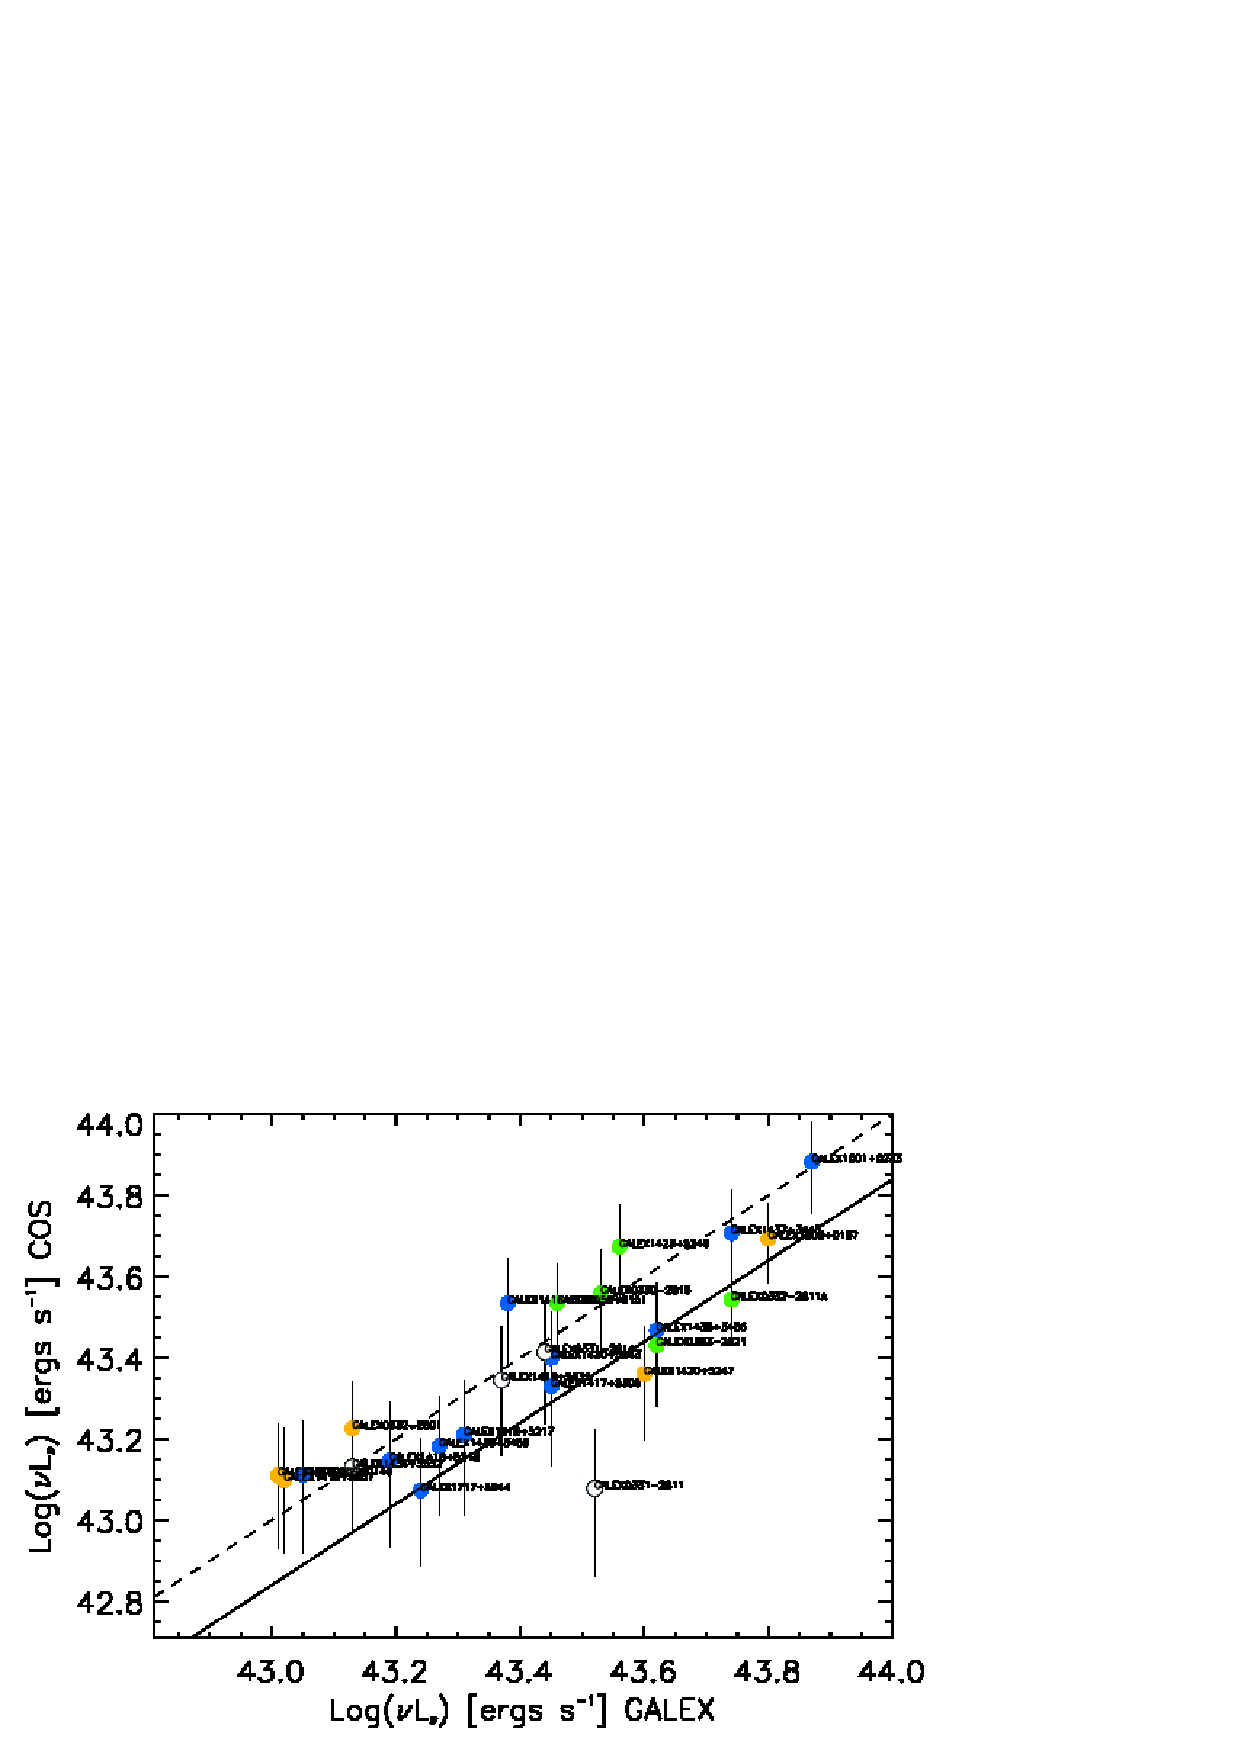
\includegraphics[scale=0.3]{/Users/claudia/PROJECTS/COS_Lya/NUV_fluxes.png}
  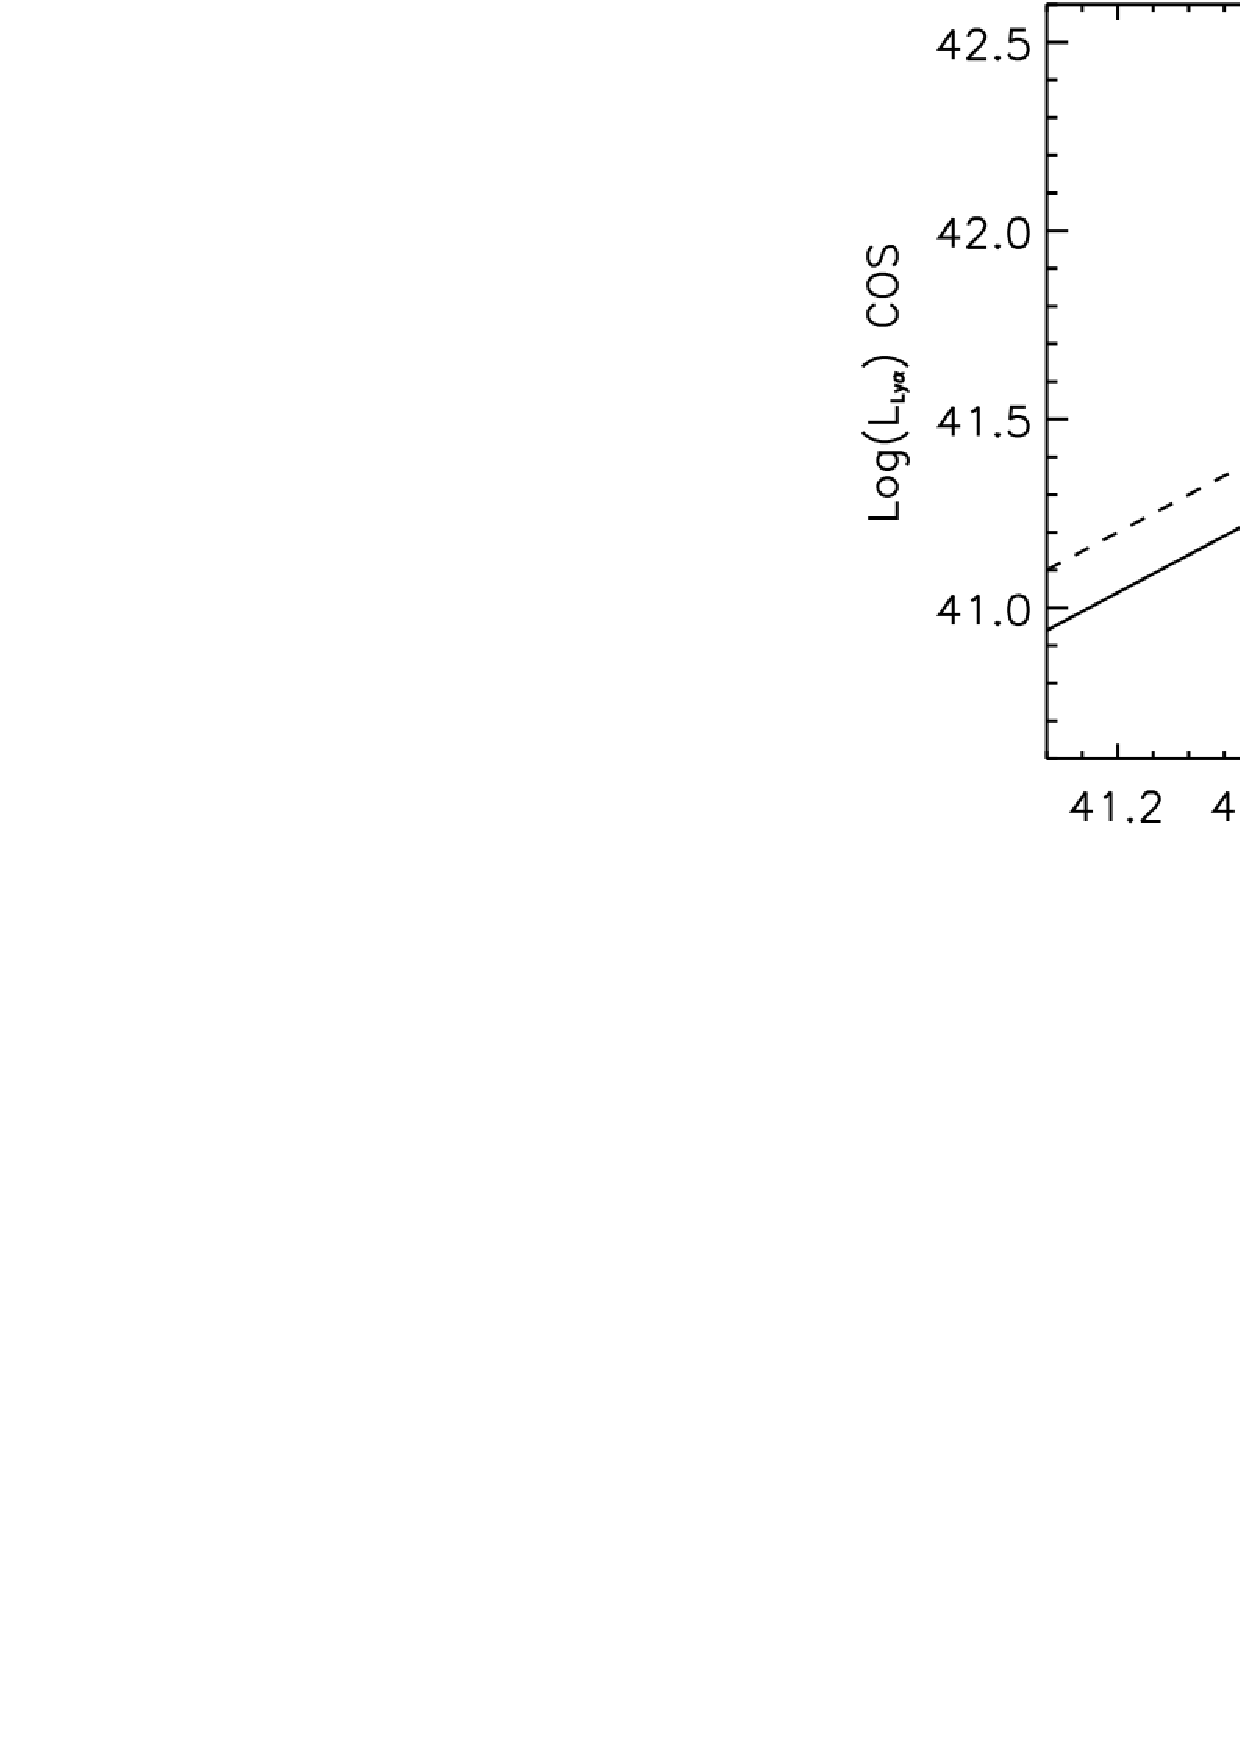
\includegraphics[scale=0.5]{/Users/claudia/PROJECTS/COS_Lya/Lya_GALEX_COS.pdf}
  \caption{Comparison between the total luminosities as measured by GALEX 
	and COS. The \emph{Left} panel shows the continuum fluxes in monochromatic
	units, while the \emph{Right} panel shows \lya. Large
    points have been corrected using the aperture correction estimated
    from the UV continuum. Open large squares indicate galaxies
    observed with MIRROR-B. After the aperture correction,
    approximately 30\% of the \lya\ flux is missed by the 2\farcs5 COS
    aperture, indicating that the \lya\ emission is more extended than
    the continuum.}
  \label{fig:GALEX_COSflux}
\end{figure*}

The PSA aperture throughput decreases toward the edges of the field of
view, due to the increasing vignetting of the flux. This change in
throughput is not accounted for in the {\tt calcos} pipeline, which is
optimized for point sources, and results in an underestimate of the
extracted flux for extended sources. We scaled the extracted spectra
by a correction factor computed using the directing imaging, and
assuming that the aperture throughput is symmetric with respect to the
aperture center. The scaling factors vary between 1.1 and 1.3. 

Because of the acquisition strategy, the vignetting correction may be
significant even for  compact sources, if the object was not perfectly centered 
within the aperture.  Figure~\ref{fig:GALEX_COSflux} (left panel) shows the 
comparison between the total aperture--corrected NUV flux measured in the 
2\farcs5 COS aperture and the GALEX NUV total flux. For each galaxy, we show the COS
measurements before and after vignetting correction, and the size of
the points is proportional to the measurement of the half-light-radius
(see below).The solid line indicates the 1:1 relation. Corrected fluxes in
the small COS apertures show a  broad agreement with the GALEX
measurements, indicating that the objects do not have substantial amount of 
light falling outside the COS aperture. We do not see a systematic trend 
with  galaxy size. We checked that for the typical NUV-I colors of
  our sources, the color term between the GALEX and COS magnitudes is
  negligible.

In Appendix~\ref{app:spectra} we show the full COS FUV segment (either A or B) covering the \lya\ profiles. 
The spectra have been binned in order to increase their signal--to--noise ratio. We chose a bin-size of 10(20) pixels 
in the dispersion direction, corresponding to XXX\AA(XXX\AA). This bin size does not substantially decrease the effective 
spectral resolution of the data, which depends on the object size (in COS native pixels) in the dispersion direction. 
We computed the errors associated with the binned profiles following the procedure described in \citet{henry2015}.
Briefly,  we used Poissonian statistic to computed the noise on the observed total counts  in each bin (from the GCOUNTS), following \citet{gehrels1986}. We then computed the errors on the flux by dividing for the exposure time and the sensitivity curve.


\subsection{Measurement of line flux and wavelength of line peak}\label{sect:peakmeas}
Figure~\ref{fig:spectra_full} shows the spectra of the GALEX sources centered around the position of the \lya\  emission line. 
The line profiles are presented in velocity space, shifted into the rest-frame using the systemic velocity calculated from 
the \ha\ emission line (see Table~\ref{tab:XXX}, for the source of the optical redshift).
The profiles are characterized by complex structures and asymmetric shapes, often with multiple peaks. 
We compute the total \lya\ flux within the aperture, by  integrating the continuum--subtracted line profile between 
$\pm 2.5$\AA\ from the expected line center. We estimated the continuum by computing the median flux density
within 2\AA\ on both sides of the line center. The line-flux error was
computed from the error spectrum derived during the spectral extraction process.  

Low spectral resolution \lya\ emission line profiles of high redshift galaxies, as well as of the majority of 
local massive galaxies show that the emission line is typically characterized by a single, broad, asymmetric peak typically 
redshifted with respect to  the galaxy systemic velocity  \citep{REF,REF}. Recent results from COS spectroscopy, however, 
showed that lower--mass, extreme emission line,  compact galaxies have \lya\  profiles characterized by both a prominent peak (redshifted w.r.t. the galaxy systemic velocity) but also a secondary emission peak, blueshifted w.r.t. the systemic velocity \citep{henry2015,jaskott201X}.

For each galaxy, we provide a measurement of the peak velocities in Table~\ref{tab:measurements}.  
 Hereafter we  follow the convention that blue(red) peak  identify the peak on the blue(red) side
of the \lya\ wavelength expected from the \ha\ redshift. We, when two peaks are present in the profile, $\lambda_R$ refers to the wavelength of 
The peak wavelengths were derived by fitting a Gaussian function to a small wavelength range ($\pm 0.6$\AA) 
centered around the visually identified position of the peaks. For the four objects for which MIRROR-B was used in 
the acquisition process, errors in the peak wavelength include the $0.1$\AA\ centering uncertainty. 
In order to compare with lower--resolution measurements we also compute the centroid wavelength of the line as:

\begin{equation}
\lambda_C=\frac{\sum{f_{\lambda}v}}{\sum{f_{\lambda}}},
\end{equation}

\subsection{Size measurement and concentration}
We use the COS images to measure galaxies' sizes in the NUV.  Because
of the complicated morphology of the star-forming regions in many of
the galaxies, we cannot fit a smooth profile to the UV light
distribution (e.g., GALEX1436$-$3456). We have therefore computed the
radius of the circular aperture containing half of the total NUV flux,
using a curve of growth analysis. The centers used for the circular
apertures are indicated with a cross in Figure~\ref{fig:images}.
Because of the small aperture of the COS instrument, we use the GALEX
NUV luminosity as an estimate of the total light of the
galaxy. Before computing the aperture flux, we multiplied each
NUV image by the COS aperture response map to account for the
decreasing throughput as function of the spatial offset from the
aperture center \citep{Goudfrooij2010}. The half--light--radii are
reported in Table~\ref{tab:info}.

\section{Results}

\subsection{UV-morphology}
Being sensitive to light between 1600 and 3100\AA, the COS NUV channel
probes the continuum coming from hot young stars.  \lya\ is inside the
NUV bandpass for only three of our galaxies, (those at at $z>0.31$),
where the EW is anyway insufficient to dominate the global light, but
could in principle extend the morphologies somewhat.
Figure~\ref{fig:images} we show the NUV COS images of the 25 galaxies,
together with the position of the circular COS aperture (when it could
be determined, see section~\ref{sec:data}). The galaxies show a
variety of morphology in the NUV: in some objects (e.g.,
GALEX1417$+$5305) the UV light is distributed smoothly over a large
part of the COS aperture (i.e., diffuse objects), in others (e.g.,
GALEX1417$+$5228) the light is concentrated in a single compact star
cluster (i.e., compact objects), while in others (e.g.,
GALEX1000$+$0157) the light is distributed in multiple clumps.  The
morphological classification is reported in Table~\ref{tab:lya}.

In Figure~\ref{fig:GALEX_COSflux} (right panel) we compare the
total, aperture--corrected \lya\ flux from the COS spectra, with the
line intensity derived in \citet{cowie2011}. For the \lya\ luminosity,
we use the vignetting correction derived from the NUV images, as
explained in Section~\ref{sec:data}. The comparison between the GALEX
and COS measurements is informative, because the two instruments have
different aperture size. The dashed lines in both panels indicates a
factor of two difference in luminosity between the GALEX and COS
measurements. It is interesting that for most of the galaxies the
\lya\ luminosity measured within the COS aperture is less than a
factor of two fainter than the GALEX measurement, while the opposite
is true for the UV luminosities. At face value, this result would
indicate that the \lya\ is more compact than the UV emission, in
contrast with the strong evidence for more extended \lya-emission in
nearby and high-$z$ galaxies presented by \citet[e.g., ]{hayes2013,
  steidelXXX, hayesXXX}. Given the uncertainty in the vignetting
corrections we do not discuss this point any further.

\subsection{Ly$\alpha$ profiles}

\begin{center}
\begin{figure*}[h!]
 \includegraphics[scale=0.5]{/Users/claudia/PROJECTS/COS_Lya/spectra2.png}
   \caption{Rest-frame COS spectra of the 25 sample galaxies around the \lya\
     emission lines. The systemic velocity is determined from the
     nebular \ha\ line. The spectra have been boxcar smoothed by 0.5\AA. }
  \label{fig:spectra_lya}
\end{figure*}
\end{center}

\begin{figure}[h!]
   \centering
   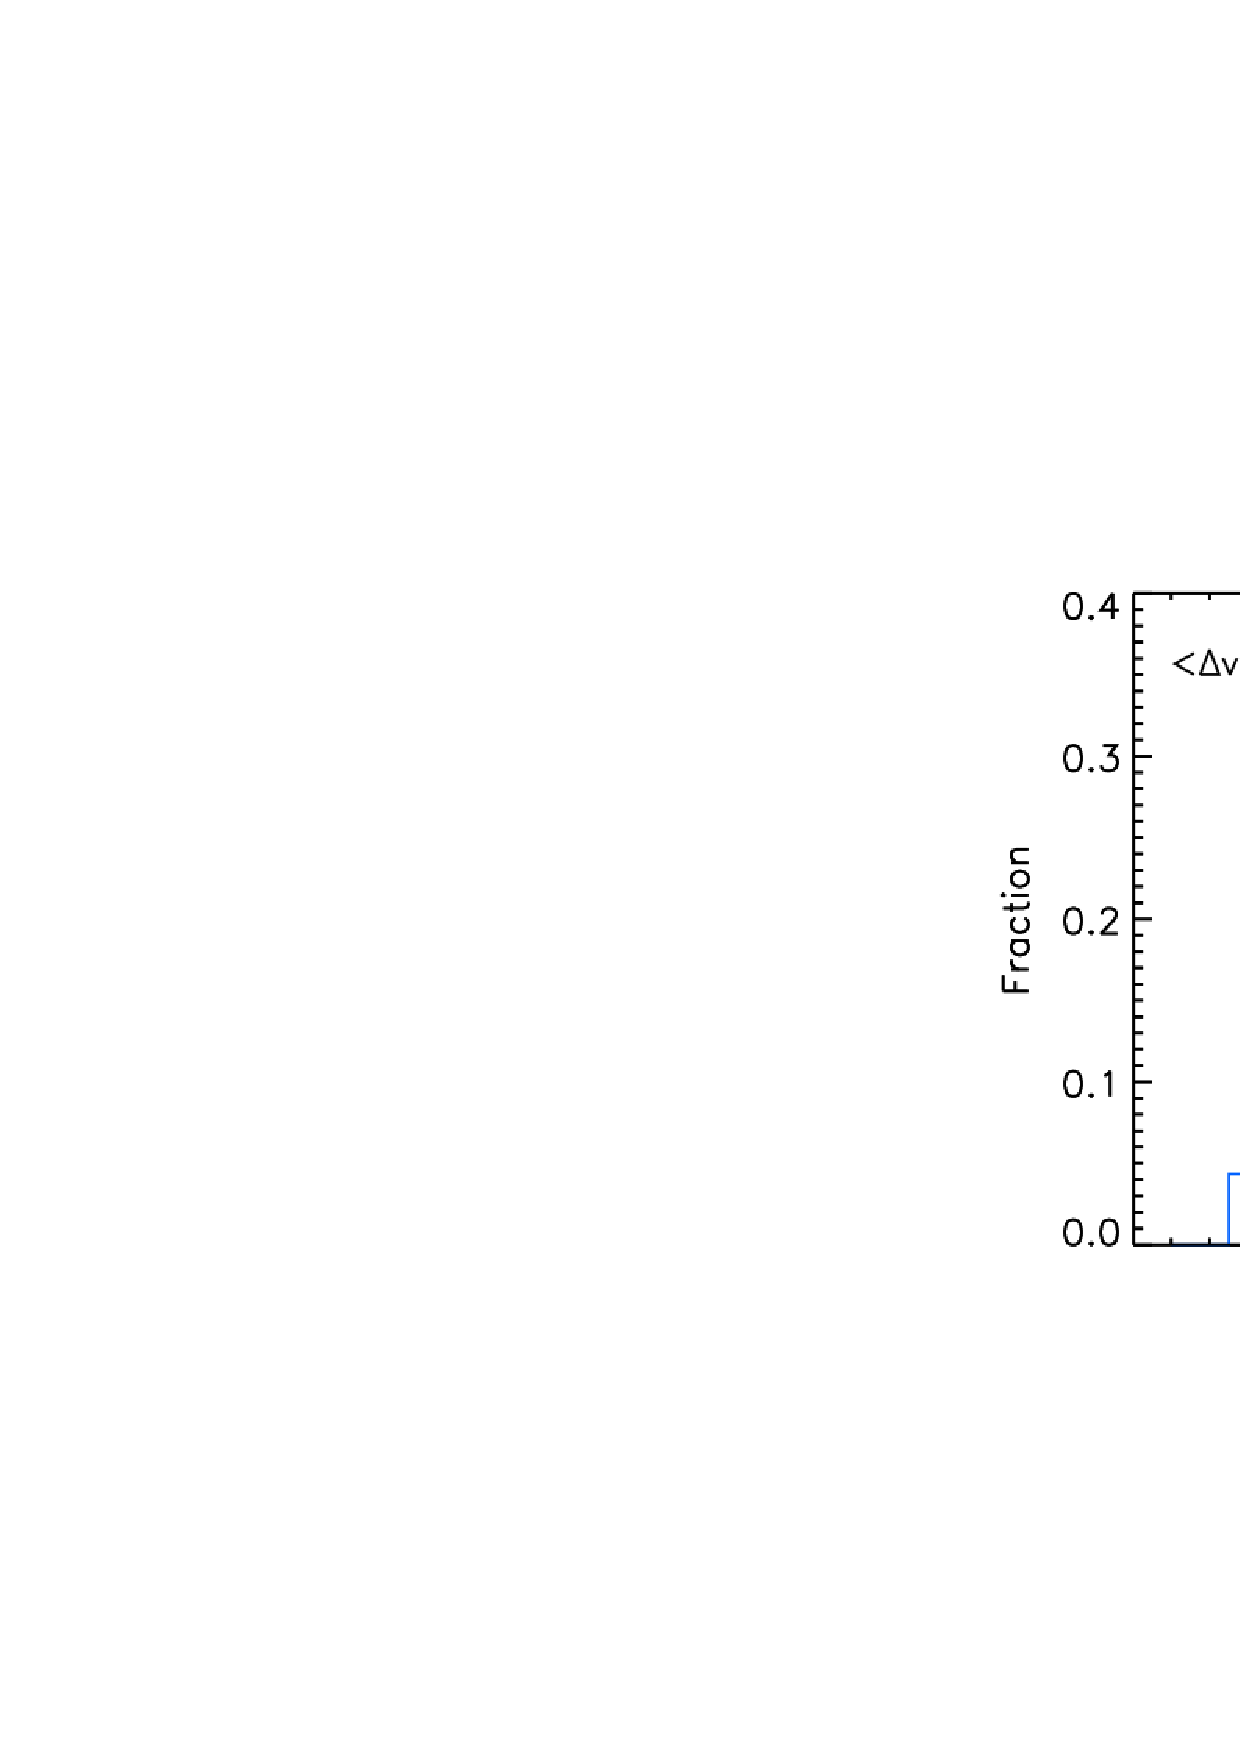
\includegraphics[scale=.35]{/Users/claudia/PROJECTS/COS_Lya/delta_v.png}
   \caption{Histogram of the velocity difference between the \lya\ and
     \ha\ line. The black solid histogram shows the shifts for our
     GALEX LAEs at $z\approx 0.2$, while the blue histogram shows the
     offsets for $\langle z \rangle=2.27$ LBGs from Steidel et al
     (2010). The arrow shows the shift of 104 km/s measuerd in the
     stacked spectrum shown in Figure~\ref{fig:stack}.}
   \label{fig:histvel}
\end{figure}

In Figure~\ref{fig:spectra_lya} we show the profiles of the \lya\
emission lines, centered on the galaxy systemic velocity derived using
the \ha\ emission line. The spectra are shown after 10 pixels ($\sim
$XXX\AA) boxcar average. In two galaxies (GALEX1418$+$5259 and
GALEX0959$+$0149) the \lya\ line is very faint, and it is detected
only after a rather heavy boxcar smoothing ($\sim 0.7$\AA).  The
vertical dashed line in each panel shows the expected wavelength
position of the \lya\ based on optical-lines redshift measurements.
In a clear majority of cases ($\sim 20$ of 25) the peak of the \lya\
line is notably offset in wavelegnth to the red of the systemic
velocity. In some cases multiple peaks are also visible, with a
tendency (at least 10 cases) to show an additional peak on the blue
side of the main peak, and also clearly bluewards of the systemic
velocity. A handful of galaxies show additional red peaks that that
are clearly separated in three cases, and also extended bumps in the
red wings of the primary line that could also be indicative of
extended red features.

Using the measured wavelengths of the strongest \lya\ emission peak,
we compute the offsets relative to \ha. These values are presented
also in Table~\ref{tab:xxx} and range generally between $-50$ and
$+350$ km/s, with a mean velocity shift of $121\pm 18$ km/s (standard
error on the mean). We present this velocity distribution in the form
of a histogram in Figure~\ref{fig:histvel}.

\subsection{Continuum properties of the sample}
The observations were designed to target the \lya\ line, and
consequently the continuum is not well exposed in individual galaxies.
In Figure~\ref{fig:spectra_full} we present the full COS spectra
shifted into the rest-frame using the redhift measured from the \ha\
emission line. The spectra are boxcar smoothed using a box of 1\AA,
and are shifted in the vertical direction for clarity.  The horizontal
dashed lines show the zero flux level corresponding to each galaxy
spectrum, while vertical lines mark the wavelength position of some
prominent interstellar absorption
features. Figure~\ref{fig:spectra_full} shows that we are able to
identify the strongest absorption feature only in a few individual
sources, although the low S/N of the spectra prevent us from performing
an accurate analysis.


\begin{figure*}[h!]
   \centering
  \includegraphics[scale=0.7]{/Users/claudia/PROJECTS/COS_Lya/continuum.pdf}
   \caption{Rest-frame full NUV spectra of the 25 sample. The spectra are boxcar smoothed us-
ing a box of 1\AA, and are shifted in the vertical direction
for clarity. The horizontal dashed lines show the zero flux level corresponding
to each galaxy spectrum. Vertical lines mark the wavelength position
of some prominent interstellar absorption features.}
  \label{fig:spectra_full}
\end{figure*}

Sample-averaged inferences can, however, be made through a stacking
analysis. We blueshift the observed spectra into the rest-frame using
the measured \ha\ velocities. At every wavelenght we compute a
flux-weighted average and standard deviation. The mean stacked UV
spectrum (shown after a box-car smoothing of 0.85\AA) can be seen in
Figure~\ref{fig:stack}, where the shaded gray area corresponds to the
weighted standard deviation, and the top panel shows the number of
galaxies that entered the stack at each wavelength.

We are able to identify and clearly measure the features presented in
Table~\ref{tab:abs} and marked in Figure~\ref{fig:stack}. The list
includes five lines that form in the ISM and one (C{\sc iii}$\lambda
1175$) that is mainly photospheric. It is reassuring that the velocity
shift of the C{\sc iii} photospheric line is consistent with zero, as
would be expected for young massive stars responsible of the
ionization of the HII regions. The ISM lines, on the other hand, all
show asymmetric absorption profiles, with the peak  blueshifted outflow velocities in the range between 150--200 km
s$^{-1}$. 

%\begin{figure*}[t!]
 %  \centering
%   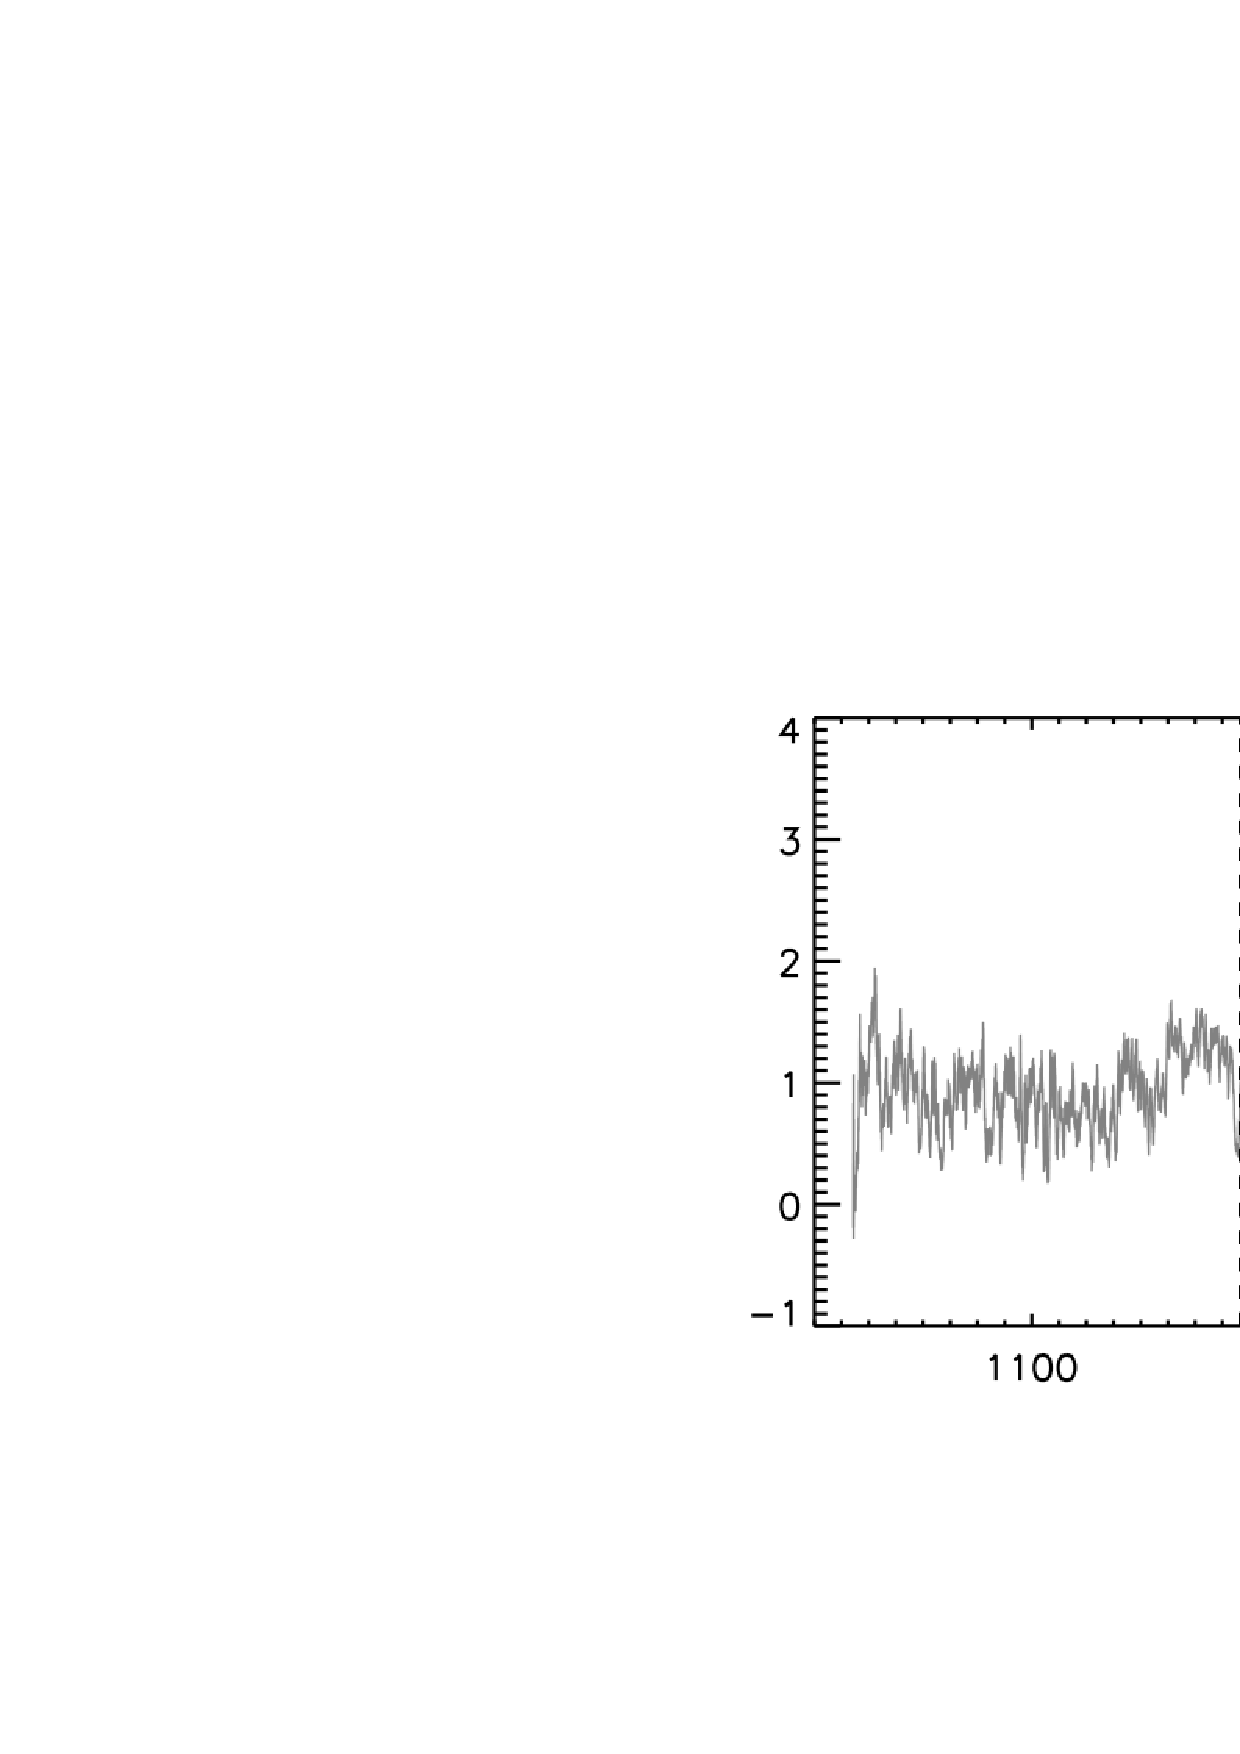
\includegraphics[scale=.5]{stack.pdf}
%   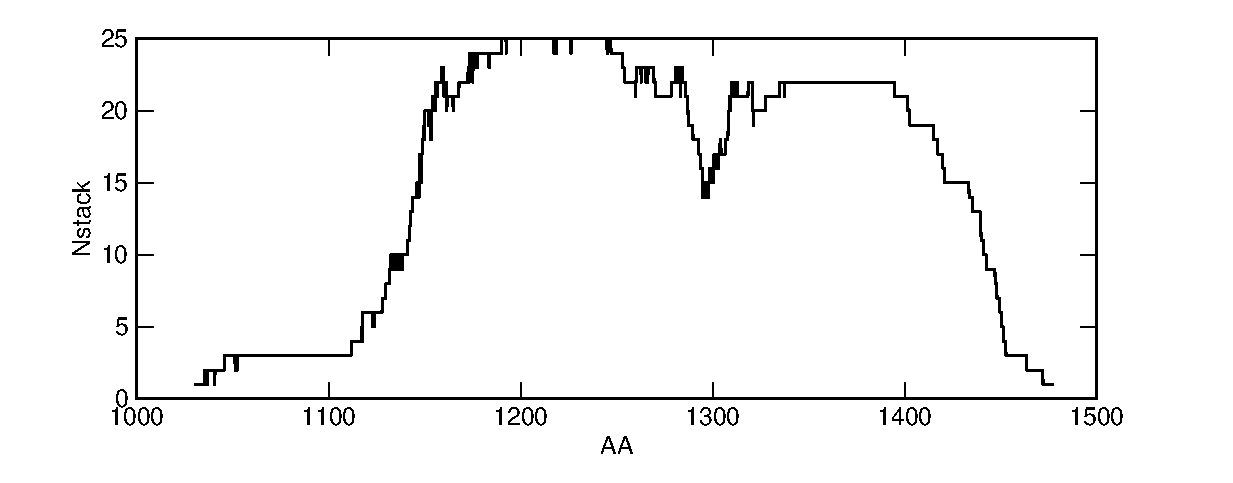
\includegraphics[scale=.6]{Nstack.eps}
%   \caption{Composite spectrum from XXX galaxies. {\bf COULD BE GOOD TO SHOW THE NUMBER OF %CONTRIBUTED FRAMES?}}
%   \label{fig:stack}
%\end{figure*}

\begin{deluxetable}{llccc} 
%\tablecolumns{5} 
%\tablewidth{0pc} 
\tablecaption{Absorption lines measured in the stacked spectrum.\label{tab:abs}}
\tablehead{ 
\colhead{Species} & Formation & \colhead{$\lambda_\mathrm{vac}$} &  \colhead{$\lambda_{\mathrm{obs}}$} &  \colhead{$\Delta V$} \\
\colhead{} & &  \colhead{\AA}   &  \colhead{\AA} }
\startdata 
H~{\sc i}~\lya & ISM   & 1215.67 & 1216.09 & 104.30 \\
%C~{\sc iii}   & Photo & 1175.59 & 1175.49 & --26.616 \\
C~{\sc iii}   & Photo & 1175.53 & 1175.37 & --39 $\pm$41 \\
%Si~{\sc ii}   & ISM   & 1190.42 & 1189.78 & --159.97 \\ this line is
%from n=0
Si~{\sc ii}   & ISM   & 1190.42 & 1189.83 & --159.97 \\ 
%Si~{\sc ii}   & ISM   & 1193.29 & 1192.60 & --173.39 \\ \\ this line is
%from n=0
Si~{\sc ii}   & ISM   & 1193.29 & 1192.60 & --173.39 \\ 
Si~{\sc iii}  & ISM   & 1206.50 & 1205.87 & --156.02 \\
Si~{\sc ii}   & ISM   & 1260.42 & 1259.56 & --205.19 \\
 Si~{\sc ii}  & ISM   & 1304.37 & 1259.56 & --205.19 \\
 C~{\sc ii}  & ISM   & 1334.53 & 1333.81 & --161.69 \\
\enddata 
\end{deluxetable}

%fine structure 1190: 1194.5,1197.39

\section{Discussion} 

\subsection{\lya\ output and UV surface density}
Smaller galaxies tend to have larger \lya\ EW
(Figure~\ref{fig:lyasize}), however, this does not seem to be a
consequence of smaller galaxies having a higher UV surface density
(Figure~\ref{fig:lyauvsd}) surface density.

\begin{figure}[t!]
   \centering
   \includegraphics[scale=.4]{/Users/claudia/PROJECTS/COS_Lya/FWHM_ew.pdf}
   \caption{\lya\ EW versus UV half light radius. Symbols as in
     previous figures. Horizontal red bars indicate the range of
     typical sizes of \lya\ emitters at different redshift as indicated.}
   \label{fig:lyasize}
\end{figure}

\begin{figure}[t!]
   \centering
   \includegraphics[scale=.4]{/Users/claudia/PROJECTS/COS_Lya/FWHM_UVd.pdf}
   \caption{\lya\ EW versus UV surface density. Symbols as in
     previous figures.}
   \label{fig:lyauvsd}
\end{figure}

\begin{figure}[t!]
   \centering
   \includegraphics[scale=.4]{/Users/claudia/PROJECTS/COS_Lya/dv_fwhm.pdf}
   \caption{The \lya-\ha\ velocity shift compared with the line width
     of the red peak of the \lya\ profile. Open circles indicates
     galaxies observed with MIRROR-B.}
   \label{fig:dvha}
\end{figure}

% Let $x$ be :
% \begin{equation}
% x=\frac{\nu - \nu_0}{\Delta \nu_D};
% \end{equation}

% \noindent
% where $\nu_D=V_{th}/c\nu_)$ is the Doppler frequency width.

% \noindent
% {\bf Homogeneous slab, monocromatic radiation} 
% What determines the shape of the output spectrum in this case are the
% temperature and the optical depth of the neutral medium.
% For a dust-free slab, the profile is double peaked and simmetric
% around $x=0$. The peak frequency in this case ($x_p$) depends on $T$
% and $\tau_0$ (the optical depth at the line center),
% with $x_p \sim \pm 0.88(a\tau_0)^1/3$. The more optically thick the
% medium is the more the peaks are separated.

% In the presence of dust, the profile does not change much.

% {\bf Expanding infalling halos}
% The \lya\ profiles resulting from a monochromatic source surroundes by
% an expanding/infalling shell of gas are perfectly symmetric to
% each other. Expanding halos present a red peak while infalling halos
% show a blue peak.
% \subsection{Radiative driven stellar winds}
% Winds==> high density==> expanding material is opaque/optically thick
% to scattering in many atominc spectral-line transitions.

\subsection{Lyman alpha scattering in galaxy outflows} 
It is frequently noted that \lya, when found in emission, presents as
a feature systematically redshifted from its systemic velocity (Kunth
et al 1998, Shapley et al 2003, Tapken et al 2004, McLinden et al
2011).  P\,Cygni-like \lya\ profiles are thought to arise by
scattering in neutral gas that has been accelerated by mechanical
energy returned from the star formation episode (Ahn \& Lee XXX,
Verhamme et al 2006). Our measured velocity shift for the interstellar
absorption lines (150--200 km/s) places our stacked galaxy somewhere
in the middle of the distribution for star-forming galaxies in the
nearby universe selected for observation with HST (Leitherer et al
2011), suggesting they are not providing extreme feedback compared to
their gas masses.  Indeed the velocity shift of the LIS absorption
lines compared with \ha\ is also very similar to the sample average of
164~km/s measured in LBGs at $z\sim 2.7$ (Steidel et al 2010).

Regarding \lya\ emission, radiative transport modeling has suggested
that characteristic offsets to \lya\ should exceed the blue-shifting
of the neutral ISM offsets by factors of around two (Verhamme et al
2008). Measuring neutral ISM lines in faint \lya-selected high-z
galaxies is usually beyond the limits of the data in most LAE
spectroscopic observations, but recently a number of \lya\ velocity
offsets have been measured with respect to \ha\ and [OIII] lines:
McLinden et al (2011) report offsets of 125 and 342 km/s for the two
galaxies; Finkelstein et al (2011) report a 162 km/s offset in one
galaxy and another that is consistent with zero; Hashimoto et al
(2012) present four more galaxies with $\Delta v_{\mathrm{Ly}\alpha}$
between 0 and 200 km/s; Guaita et al (submitted) present four more
galaxies with offsets between 100 and 350~km/s. Our sample of 25
$\langle z\rangle=0.2$ LAEs is twice the size of the combined samples
at $z=2-3$ and find a very similar distribution of \lya\ velocity
offsets, and suggests this offset to be somewhat characteristic of the
\lya-selected galaxy population, independent of redshift.

Similarly made measurments in continuum-selected galaxies at $z\sim 2.7$
find average absorption line offsets that match that measured in
our stacked spectrum with surprising accuracy. It is of marked interest, 
therefore, that \lya-\ha\ offsets measured in the same sample of almost 100
LBGs (Steidel et al 2010, see also Kulas et al 2012) find a an average 
$\Delta v_{\mathrm{Ly}\alpha}$ four times the value that we measure in the 
more nearby Universe. While the average offset of \lya\ compared with the LIS lines for LBGs appears 
consistent with predictions from radiative trasport models our average 
measurement of a \lya\ offset significantly below the LIS offset is in stark
contrast to predictions. 

A plausible reconciliation of \lya\ shifts below the outflow 
velocities of the oncoming gas may lie in exactly where in the HI medium
\lya\ obtains its redistribution in frequency.
A measurement of the LIS lines will return the velocity at which the column 
density of the absorbing species -- and presumably also neutral hydrogen -- 
is highest. For typical column densities in star-forming galaxies this may 
be on the order of $10^{20}$ cm$^{-2}$ (Mas-Hesse et al 2003). In static 
gas, \lya\ becomes optically
thick at column densities roughly 6 orders of magnitude below this value, which 
suggests that the gas responsible for the frequency distribution is both of lower
column density and velocity than the bulk of the outflowing gas, and also resides 
closer to the recombination nebulae. Yet this scenario is not able to explain
the marked difference seen between the \lya\ and UV selected populations: why
should the situation be different in the two populations? It is plausible also 
that we are observing the transition between \lya\ photons that have been 
backscattered from receeding shells (which must acquire around twice the
velocity shift of the outflowing gas) and photons that are able to pass directly
through the oncoming shell. The multiple peaking of many of the \lya\ profiles 
is indeed also suggestive of this: indeed it appears that we are observing 
a large number of double-peaked profiles, in which the red peak is enhanced 
compared to the blue. From the available publications of transport modeling, 
this seems most resemblant of photon transfer and frequency redistribution
in a single front-side medium. 

\subsection{What drives the velocity shift?} 

If the \lya\ velocity shift is present, and the neutral gas observed to 
be accelerated, then one may expect the feedback to be coupled with other
properties of the star-formation episode. 
 Specifically, for example, outflows may be stronger in 
galaxies of higher SFR or specific SFR which in turn may manifest in 
larger velocity offsets. Adopting the \ha\ luminosity as a proxy for SFR
and its equivalent width as a rougher proxy for sSFR, we present the \lya\ 
velocity shift compared with L(\ha) and EW(\ha) in the upper two panels
of Figure~\ref{fig:dvha}. 

\begin{figure}[t!]
   \centering
   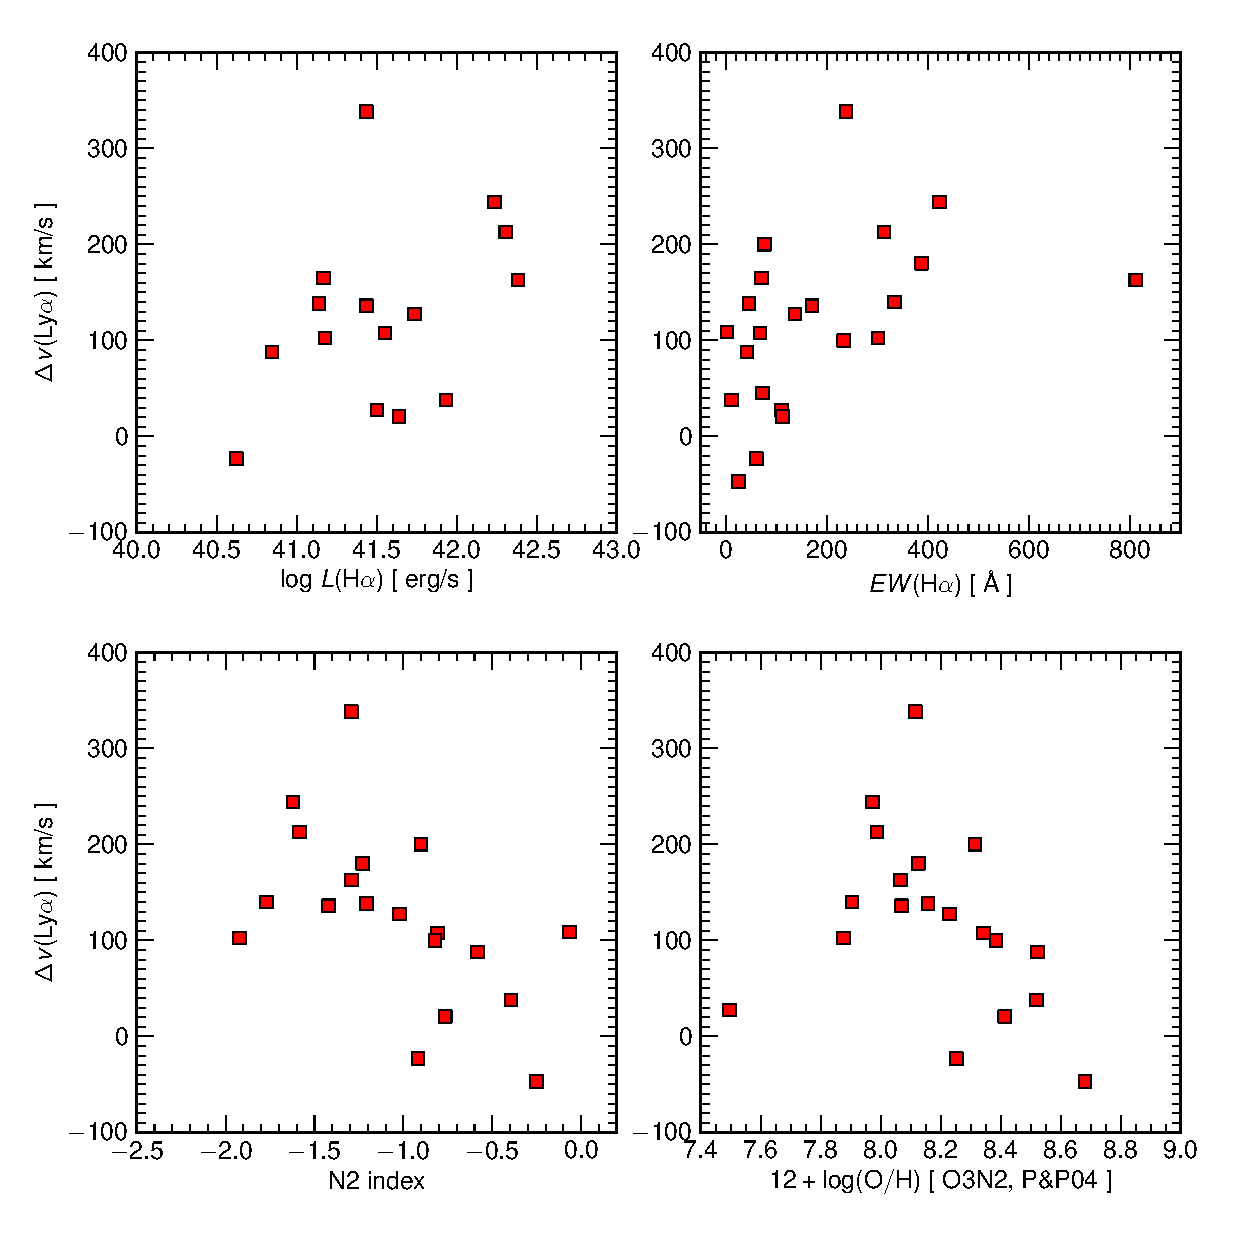
\includegraphics[scale=.4]{dvel_ha.eps}
   \caption{The \lya-\ha\ velocity shift compared with 
			 (a. \emph{Upper left}) the \ha\ luminosity; 
			 (b. \emph{Upper right}) \ha\ equivalent width; 
			 (c. \emph{Lower left}) N2 index; 
			 (d. \emph{Lower right}) gas phase metallicity }
   \label{fig:dvha}
\end{figure}

The data present no such correlation of offset with SFR. Indeed while 
higher SFR must imply that more mechanical energy has been fed back to 
the ISM, it does not necessarily mean that the outflow would be faster. 
SFR and stellar mass are known to be strongly correlated 
in almost all galaxy samples, and should the neutral gas mass also scale
with stellar mass, proportionally more energy would be needed 
to drive a superwind of the same velocity. In this picture, a correlation 
with SFR would not be expected, but one would expect a stronger velocity 
offset when the SFR per unit mass, or sSFR, increases. Interestingly, then, 
the plot of $\Delta v(\mathrm{Ly}\alpha)$ against $EW(\mathrm{H}\alpha)$ shows 
a marked lower envelope consistent with this formulation. Galaxies with low 
equivalent widths ($\lesssim 100$\AA) can 
take the full range of outflow velocities (0 -- 200 km/s), whereas galaxies with
high sSFR ($EW$(\ha) $>200$~\AA: eight of 22 measureable galaxies) present only 
with $\Delta v(\mathrm{Ly}\alpha)$ 
above the sample average value of 100 km/s.  It is plausible
therefore, that since these galaxies have high SFR compared with their stellar mass, 
their SFRs may also be high compared with their neutral gas mass and are able to
push the \lya\ scattering medium to higher velocities. 

From the optical spectra we also compute the N2 index 
[$\equiv$ log$_{10}$(\nII6584/\ha)] and the gas-phase metallicity which we derive 
from the O3N2 index using the strong line calibration of calbiration of 
(Pettini \& Pagel 2004). Here also there appears to be a rough anti-correlation 
between $\Delta v(\mathrm{Ly}\alpha)$ and {N2,O/H}. However we note that the 
emission line measuements involve no quantitiy sensitive to the mass of the stellar 
population. Metallicitiy does, however, correlate strongly with stellar mass, 
implying that velocity shifts are somewhat higher in lower mass objects. 
This aligns well with the reasoning presented above, in explaining how a large 
range of offsets may be observed, despite showing no overall correlation with 
the total star formation rate. 

\subsection{How would a neutral Universe effect these observations?}

In high-redshift studies, \lya\ fluxes, number counts, luminosity functions, 
and asymmetries are all thought to be affected by the increasingly neutral 
fraction of hydrogen in the neutral IGM. However, disentangling possible IGM
effects from those of the ISM has never been possible in these galaxy samples. 
In our $\langle z\rangle=0.2$ observatations we can perform a number of 
comparison studies on a set of observations for which we can be certain that 
the IGM has no influence on the \lya\ line. We now proceed to examine how 
common assumptions about the IGM affect \lya\ photometry and measurments of the 
profile asymmetry. 


\subsubsection{Photometry in an ionized and neutral universe}

One of the primary use of the \lya\ line in astrophysical cosmology is as a 
diagnostic of the reionization epoch, as an increasingly high fraction of 
intergalactic gas becomes neutral with increasing redshift 
(Miralda-Escude 1998; Haiman \& Spaans 1999; Malhotra \& Rhoads 2006; 
Kashikawa et al. 2006). Furthermore, should one want to derive the 
intrinsic \lya\ output of a galaxy (before IGM attenuation) one needs to
correct for the IGM. Indeed frequently, simple prescriptions (e.g. Madau 2005) 
for the IGM are applied directly to the \lya\ line to make this correction 
(Cassata et al 2011; Blanc et al 2011), which accounts for almost 50\% of the 
\lya\ flux at $z=6$. This is the entire premise for the recent claim of an 
extremely high EW \lya\ emitter at $z=6.5$ (Kashikawa et al 2012). 
These corrections include two major unknown questions: 
by how much is the \lya\ line offset redward of its systemic velocity? and 
how close do the \lya\ forest clouds really come to the \lya\ line? With these
data we have already answered the former question, and we will now proceed with
a simple assessment of how common assumptions of the latter may affect 
conclusions. 

Using the systemic redshift for our sample as measured by \ha\ and the 
canonical prescription for intergalactic Lyman series line blanketing 
of Madua (1995), we simulate or \lya\ spectra in the common redshift windows 
of $z=5.7$ and $6.5$. We simply blueshift the galaxies to $z=0$ and redshift
them to the high-z windows, apply the IGM, and re-compute the luminosities 
using the same method as in Table~\ref{tab:measurements}. We present the 
luminosities, both unattenuated and suppressed by the $z=5.7$ and 6.5 IGM, 
in Table~\ref{tab:hiz_asym}, and make a graphical comparison in 
Figure~\ref{fig:igmlum}. 

\begin{figure*}[t!]
   \centering
   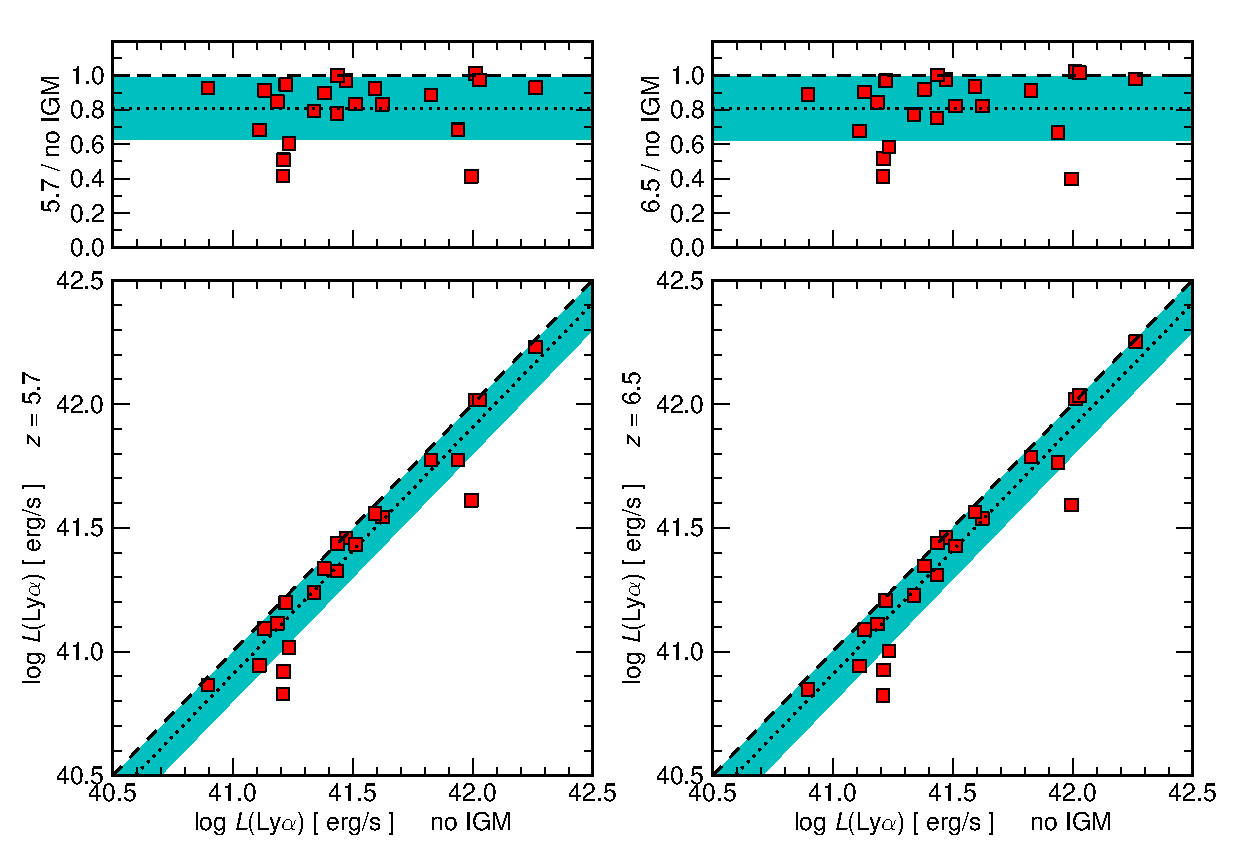
\includegraphics[scale=.65]{lumcomp_igm.eps}
   \caption{Comparison of the measured luminosity of \lya, with the same measurements 
	when the spectra have been `absorbed' by the standard Madau (1995) IGM  prescription
	 assuming redshift $z=5.7$ (\emph{left}) and $z=6.5$ (\emph{right}). The lower panels
	 show a direct comparison of the luminosities, while the upper panels show the 
	 fractional luminosity that is transmitted through the IGM. By eye the \emph{left} 
	and \emph{right} plots are indsitinguishable. The dotted lines show the average 
	ratios of $L\{5.7,6.5\} = 0.81L(z=0)$, which differ only at the fourth significant 
  digit. Shaded regions show the standard error on the mean, which is almost consistent
	with the 1:1 line. 
\vspace{5mm}	 }
   \label{fig:igmlum}
\end{figure*}

Immediately it can be seen that the simulated high-$z$ luminosities lie very close 
to the total measured fluxes. Only in a handful of cases -- obviously the few 
galaxies with symmetric \lya\ lines centred around the systemic velocity -- is there
a significant suppression of the \lya\ line by the IGM. Indeed the majority of \lya\
profiles shown in Figure~\ref{fig:spectra_full} are noteably redshifted, with only 
a small component to the total flux provided by the blue peak. The effect of the IGM 
is essentially to completely remove the blue peak but leave the redshifted, dominant 
peak almost completely unaffected. We compute the average values of 
$L$(\lya,IGM) / $L$(\lya,noIGM), which evaluates to $0.81 \pm 0.17$ (standard error 
on the mean) at both tested redshifts. It is possible that additional flux could be 
suppressed by the red damping wing of a neutral IGM that has not been accounted for 
by these models. This would further suppress our \lya\ luminosities in the simulated 
spectra, but it should be noted that this is not usually accounted for either by 
high-$z$ observational studies. The damping wing would have equal additional effect 
on high-$z$ data and these simulations. With so many galaxies lying close to the 
1:1 line, we find no argument for doubling observed $z\gtrsim 6$ fluxes, especially
in individual cases. This conclusion is also supported by the fact that asymmetries
do not differ at high- and low-$z$, as we will discuss in the next section.



\subsubsection{\lya\ asymmetry in an ionized universe}

As well as applying a redward velocity offset to the transferred \lya\ line, 
scattering in netural gas is also well-known to introduce asymmetries to the 
profile itself.  In the spectra of high-$z$ 
galaxies, when spectral resolution permits, \lya\ almost ubiquitously 
presents asymmetrically (Shapley et al 2003; Kurk et al. 2004; 
Shimasaku et al 2006) and, at the highest redshifts, is expected to be
enhanced by neutral gas in the IGM. Indeed, quantitative measurements of
the profile asymmetry have also been invoked to discriminate between 
\lya\ emitting galaxies and foreground interloperes (e.g. [OII] emitters
where the line is not subject to radiative transport effects; Kashikawa 
et al 2006). As with the transmitted line flux, however, the effect that
the IGM has on the transmitted line is strongly dependent upon how close
the IGM comest to the \lya\ line that is transported through the ISM. 

\begin{figure*}[t!]
   \centering
   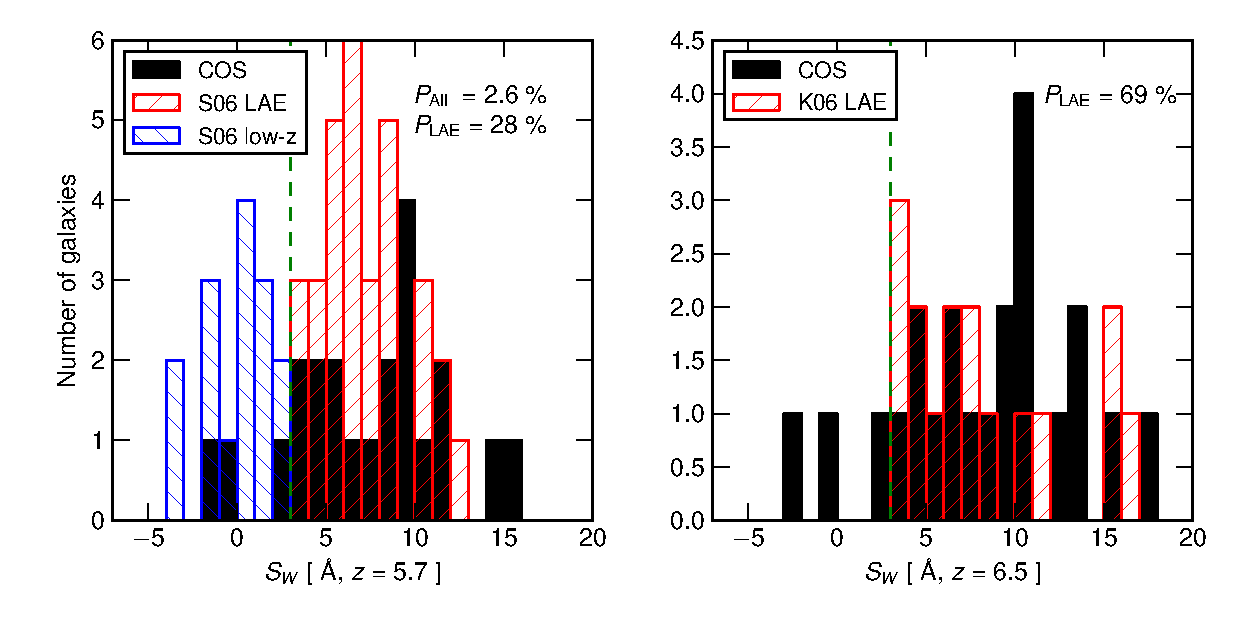
\includegraphics[scale=.8]{asym_hist.eps}
   \caption{Distribution of the weighted skewness $S_W$ of our COS \lya\ 
	profiles. Histograms of our own sample are presented in black, scaled 
	in redshift to $z=5.7$ (\emph{left}) and 6.5 (\emph{right}). Overplotted
	in the \emph{left} panel are the LAEs from Shimasaku et al (2006) in red,
 and the emission line objects determined to be lower redshift interlopers in
	blue. In the right panel the red histogram shows the LAEs of Kashikawa et
	al (2006). Labeled in the figures are the probabilities that the 
	high-$z$ samples ($z=5.7$ LAEs, LAEs+interlopers, and $z=6.5$ LAEs) are drawn
	from the same parent population using the $K-$sample Anderson-Darling rank
	sum comparison. It shows the LAEs populations to be indistinguishable but 
	LAE+interlopers are clearly unlikely to share an underlying distribution.
	 }
   \label{fig:skew}
\end{figure*}

Our well resolved and high $S/N$ COS observations give us the possibility
to compute quantitative asymmetries for a sample of \lya\ selected galaxies
in which we can say with certainty that the frequency redistribuion occurs 
inside the ISM. We opt to measure profile skewness (Kurk et al 2004), 
`weighted skewness' (Shimasaku et al 2006) and red/blue ratios of the 
peak-to-10\% wavelength and flux (Rhoads et al 2003). We are able to perform
these measurements in 22 of our 25 objects, and present the resutls in 
Table~\ref{tab:hiz_asym}. 

Firstly regarding weighted skewness, the index has been used by Shimasaku 
et al (2006) at $z=5.7$ and Kashikawa et al (2006) at $z=6.5$ to cull 
interloping galaxies from their sample, by invoking a threshold $S_W$ of $>3$ 
to select LAEs. Scaling our measurments of $S_W$ into the observer frame at
these redshifts we present histograms of the $S_W$ for the COS sample in
Figure~\ref{fig:skew}. Overplotted are the LAE and low-$z$ samples of Shimasaku, 
and LAEs measured and compiled in Kashikawa et al. It is immediately clear from
these histograms that our GALEX-selected LAEs exhibit a very similar range of 
$S_W$ to both high-$z$ LAEs samples, whereas the interloping sample of 
Shimasaku et al (2006) shows very little clear overlap. In order to assess 
this similarity quantitatively, we employ a $K-$sample Anderson--Darling (1952) 
rank sum comparison \footnote{The A--D test is similar to the frequently adopted
Kolmogorov–Smirnov (K--S) test but  considers the full range of data values as 
opposed to the largest single deviation, and is therefore more robust against
strong biases from outlying points.}. Indeed for the two LAE samples, data are 
consistent with the null hypothesis (that the two samples are drawn from the 
same parent distribution)  at only the 28\% level ($z=5.7$) and 69\% ($z=6.5$)
level. However the same test performed on the concatenated LAE+interloper 
sample at $z=5.7$ suggests there is a $<3$\% chance the the two samples 
share the same parent distribution, and the selection of $S_W>3$ as invoked
in those studies seems appropriate. It seems likely, however, that the asymmetry
is introduced by the scattering of \lya\ photons within the ISM of these galaxies
and not by an encroaching neutral IGM. If the IGM does not have an appreciable 
effect of the asymmetry of the \lya\ line at high-$z$ it must reflect the fact
that the \lya\ forest does not come cloes enough to \lya\ to sufficiently 
affect the blue wing, possibly becuase of redshifting within the ISM, which is
certainly very consistent with a reduction in flux of only $\sim 20$~\% as shown
in the previous Section. If it has an effect at all, it must be very grey, and 
likely be caused only by the damping wing. 



\begin{figure}[t!]
   \centering
   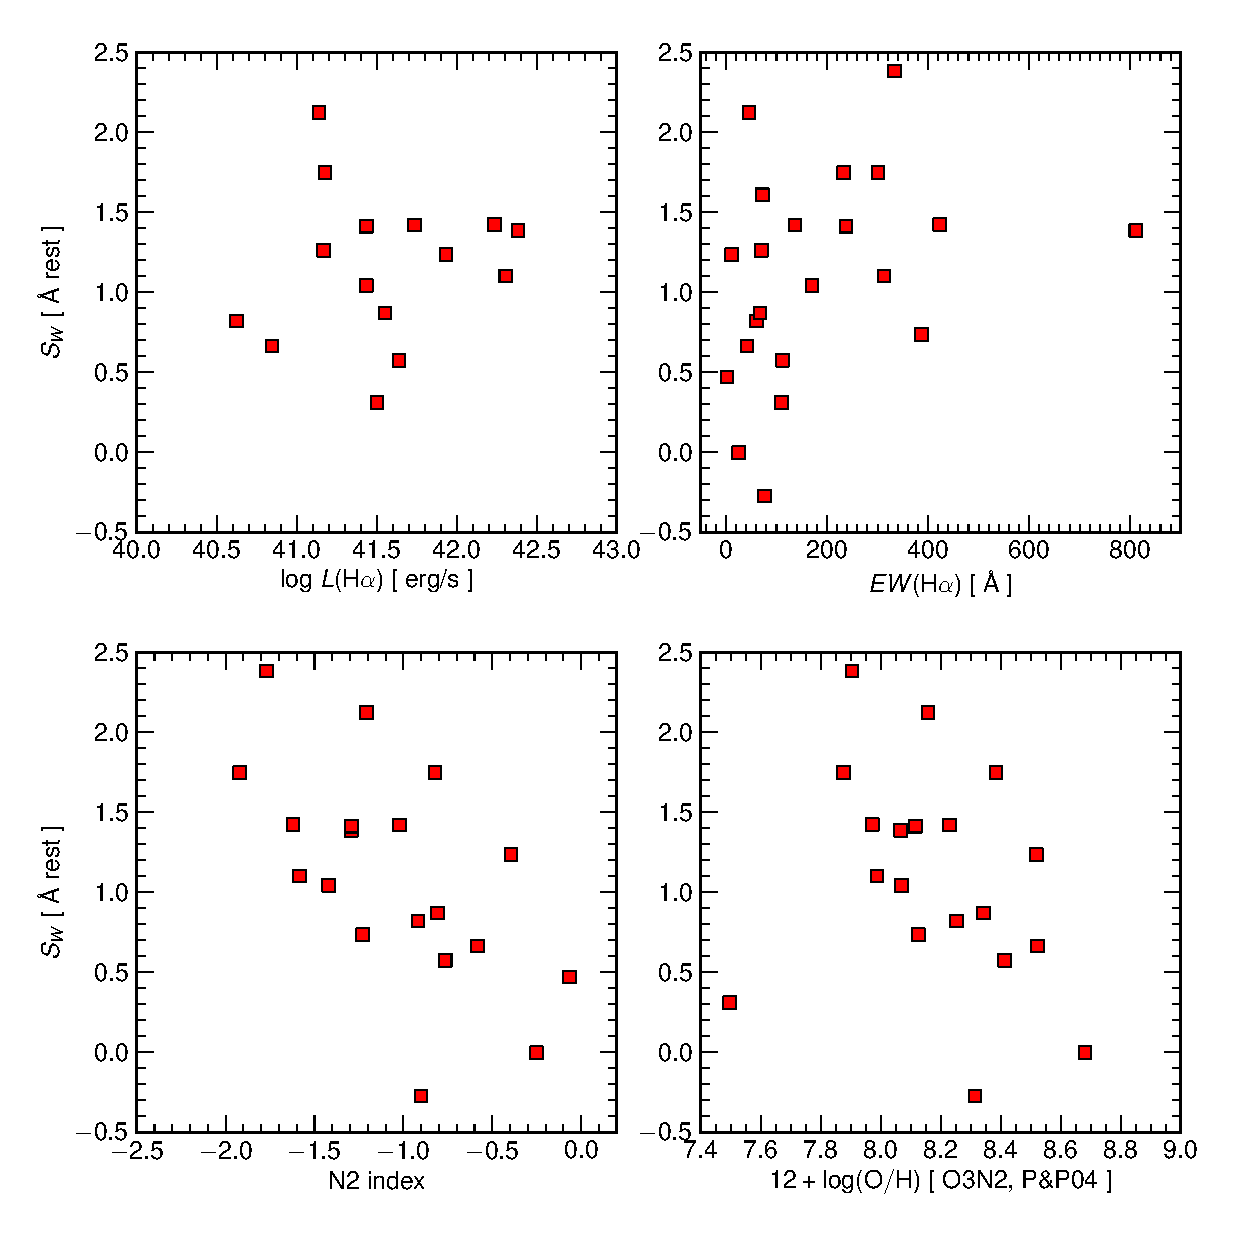
\includegraphics[scale=.4]{swr_ha.eps}
   \caption{ Same as Figure~\ref{fig:dvha} but with weighted skewness,$S_W$. }
   \label{fig:asymha}
\end{figure}




\section{Simple model for the neutral gas kinematics}


==> outflows a grandi distanze?
==> prochaska non trova il transverse proximity effect.
==> Lya nebulae su scale 

\subsection{Mass outflow rate}
We can use the best-fit parameters for the asymmetric outflow model to
estimate the average mass outflow rate $(\dot{M})$ in \lya\ emitters.
For a mass flux, and assuming that the absorbing material has a
covering fraction of one, the mass density at $r$ can be written as a
function of the gas velocity and mass loss rate ($\dot{M}$) through
the solid angle $\Omega$ \citep[e.g.,][]{martin2013}:

\begin{equation}
\rho(v)=\frac{\dot{M}}{\Omega vr^2}.
\label{eqn:density}
\end{equation} 

At $r=R_{SF}$ we have $\dot{M}=\rho_{R_{SF}} \Omega \, v_{0} \,
R^2_{SF}$. The density in the above Equation is the total gas density
($\rho=n_H m_H (1+4Y_{He})$, where $m_H$ is the mass of the hydrogen
atom, and $Y_{He}$ is the relative abundance by number of He with
respect to hydrogen).

The hydrogen number density ($n_{H}$) can be derived from the number
density of $\rm Si^+$ if the $\rm Si^+$ ionization fraction
($\chi(r)$), relative abundance with respect to hydrogen ($A(r)$), and
finally its depletion fraction on dust grains ($D$) are known.  We can
write:

\begin{equation}
n_{0,H}=\frac{n_{\rm 0,Si^+}}{\chi\,A\,D},
\end{equation}

\noindent 
where the subscrict $0$ indicates that the quantities are computed at
$R_{SF}$.  We proceed to compute $n_{\rm 0, Si^+}$ from the best--fit
value of $\tau_{0}$ (see Eqn~\ref{eqn:tau0}). The UV sizes were
computed using the COS NUV acquisition images, and range between 0.5
and 4.6 kpc, with an average value of $R_{SF}=2.1$kpc. Assuming the
average value for $R_{SF}$, we find $n_{\rm Si^+}\approx 4.4\times
10^{-7}$ cm$^{-3}$.


The depletion of Si on dust grain is uncertain. However, it is
probably low in the high velocity gas probed by our study \citep[see
][for depletion values in high velocity clouds in the Milky
Way]{savage1996}. We set $D=1$ in our calculations.

For the \lya\ emitting galaxies included in the stacked spectrum
optical spectroscopy was obtained to constrain the metal content in
the ionized--gas. Following \citep{cowie2011}, we used the $N2$
parameter ($ N2= log (f([N II]\lambda6584)/f(H\alpha)$), together with
the \citet{pettini2004} calibration derived from local galaxies.  The
average $N2$ in the sample galaxies is $-1.1 \pm 0.6$, corresponding
to an oxygen abundance of $12 + log (O/H) = 8.26 \pm 0.34$ \citep[i.e,
approximately one third solar,][]{prieto2001}. We assume that the
metallicity of the outflowing material probed by the \siii\ absorption
is the same of the ionized gas probed by the \ha\ emission. There is,
however, the possibility that the current star formation episode is
fueled by low metallicity gas accreted from the IGM.  In this case,
the outflow could potentially have a larger metallicity and 1/3 solar
can be interpreted as a lower limit. From the solar photospheric
abundance of Si relative to H given in \citet[][$n_{Si}/n_H=3.2\times
10^{-5}$]{asplund2009}, we adopt $A=1.1\times 10^{-5}$.

We can constrain the ionization state of Si ($\chi$) from the
numerical density of $\rm Si^{++}$. The latter can be estimated from
the observed \siiii\ resonant transition at 1206\AA. As shown in
Figure~\ref{fig:gaussian} the profile around 1206\AA\ is of pure
absorption, blueshifted with respect to systemic velocity by $188\pm
20$ \kms. We can reproduce this absorption profile with the same
best--fit gas geometry, density and velocity fields derived from the
\siii\ doublet, only if we do not include the scattered blue emission
(the dotted line in Figure~\ref{fig:siii1206} shows the model 
including the blue scattered re--emission). This possibly indicates
that the ratio $\rm Si^{++}/Si^{+}$ is not constant in the envelope,
and thus $\rm Si^+$ and $\rm Si^{++}$ may have different radial
density profiles. Neglecting the blueshifted re--emission results in
an underestimate of the $\rm Si^{++}$ density, by a factor of a
few. The best-fit absorption profile is shown in
Figure~\ref{fig:siii1206} (blue line). With the same $R_{SF}=2$ kpc
assumption, we find $n_{\rm Si^{++}}\approx 1.8 \times 10 \times
10^{-7}$ cm$^{-3}$, so that $n_{\rm Si^+}\approx 3 \times n_{\rm
  Si^{++}}$. Thus, we take $\chi = XXX$ in the calculation of the
total gas density. We also note that, given the relative ionization
potentials of Si (8.16 eV) and $\rm Si^+$ (16.3 eV) compared to H, the
measured $n_{\rm Si^+}/_{\rm Si^{++}}$ ratio also implies that the
observed absorption is associated with hydrogen in neutral form, and
thus the $\rm Si^+$ ions trace the neutral phase of the wind around
the star-forming regions.

Following the above discussion, we obtain a neutral hydrogen number
density at $R_{SF}$ of 0.12 cm$^{-3}$, and a corresponding mass
outflow rate from Eqn~\ref{eqn:density} $\dot{M} \approx 6 M_{\odot}$
yr$^{-1}$.

From the mass outflow rate computed above and the galaxies' average
star-formation rate (SFR), we can constrain the outflow mass loading
factor \citep[$\eta=\frac{\dot{M}}{SFR}$][]{dave2012}. In galaxy
formation models, this parameter is used to quantify the strength of
ejective feedback, which regulates both the shape of the
mass-metallicity relation, as well as the stellar mass growth rate of
low mass haloes \citep{dave2012,shen2012}. Theoretical analysis
reproducing the $Z-M$ scaling currently favor $\eta \propto
M_{*}^{-1/3}$, as expected from momentum-driven winds. However, the
value of $\eta$ and its dependence on redshift and galaxy halo mass
are still poorly constrained observationally
\citep[e.g.][]{martin2013}.

All galaxies in the sample have measured \ha\ and \hb\ luminosities
from \citet{atek2014,cowie2011,scarlata2009}. We corrected the
observed \ha\ luminosities for the dust extinction derived from the
Balmer ratio, following
% $L_{H\alpha , intr}=L_{H\alpha , obs}10^{0.4A_{H\alpha}}$, where $A_{H\alpha}=3.33\pm 0.8
% \rm E(B-V)$ and
% E(B-V)$=1.97log((H\alpha/H\beta)_{obs}/(H\alpha/H\beta)_{intr})$
\citet[e.g.][]{dominguez2013}. The average extinction corrected \ha\
luminosity for the sample galaxies is $L_{H\alpha , intr} =2\times
10^{42}$ ergs s$^{-1}$, corresponding to a star formation rate (SFR)
of 5.3 $M_{\odot}$ yr$^{-1}$ \citep[][]{kennicutt2012}.  Consequently,
the average mass outflow rate is comparable to the average SFR of the
galaxies, implying a mass loading factor $\eta \approx 1$. 






\section{Conclusions}

\bibliographystyle{apj} 
\bibliography{mybib}

\appendix
%
%\begin{figure}[t!]
%\includegraphics[scale=.25]{/Users/claudia/PROJECTS/COS_Lya/FIGURES/GALEX1417+5228_spec.png}
%\caption{ COS G160M spectrum of GALEX1417$+$5228. Red bars indicate the expected wavelength of ISM features in the galaxy, while green bars show the position of Milky Way absorption lines.TO BE DONE: geocoronal emission.}
%\label{fig:app1}
%\end{figure}
%
%\begin{figure}[t!]
%\includegraphics[scale=.25]{/Users/claudia/PROJECTS/COS_Lya/FIGURES/GALEX0331-2814_spec.png}
%\caption{  Same as Figure~\ref{fig:app1}, but for GALEX0331$-$2814}
%\end{figure}
%
%\begin{figure}[t!]
%\includegraphics[scale=.25]{/Users/claudia/PROJECTS/COS_Lya/FIGURES/GALEX0332-2801_spec.png}
%\caption{  Same as Figure~\ref{fig:app1}, but for GALEX0332$-$2801}
%\end{figure}
%
%\begin{figure}[t!]
%\includegraphics[scale=.25]{/Users/claudia/PROJECTS/COS_Lya/FIGURES/GALEX1418+5307_spec.png}
%\caption{  Same as Figure~\ref{fig:app1}, but for GALEX1418$+$5307}
%\end{figure}
%
%\begin{figure}[t!]
%\includegraphics[scale=.25]{/Users/claudia/PROJECTS/COS_Lya/FIGURES/GALEX0332-2811A_spec.png}
%\caption{  Same as Figure~\ref{fig:app1}, but for GALEX0332$-$2811A}
%\end{figure}
%
%\begin{figure}[t!]
%\includegraphics[scale=.25]{/Users/claudia/PROJECTS/COS_Lya/FIGURES/GALEX1436+3459_spec.png}
%\caption{  Same as Figure~\ref{fig:app1}, but for GALEX1436$+$3459}
%\end{figure}
%
%\begin{figure}[t!]
%\includegraphics[scale=.25]{/Users/claudia/PROJECTS/COS_Lya/FIGURES/GALEX1418+5259_spec.png}
%\caption{  Same as Figure~\ref{fig:app1}, but for GALEX1418$+$5259}
%\end{figure}
%
%\begin{figure}[t!]
%\includegraphics[scale=.25]{/Users/claudia/PROJECTS/COS_Lya/FIGURES/GALEX1001+0233_spec.png}
%\caption{  Same as Figure~\ref{fig:app1}, but for GALEX1001$+$0233}
%\end{figure}
%
%\begin{figure}[t!]
%\includegraphics[scale=.25]{/Users/claudia/PROJECTS/COS_Lya/FIGURES/GALEX1437+3445_spec.png}
%\caption{  Same as Figure~\ref{fig:app1}, but for GALEX1437$+$3445}
%\end{figure}
%
%\begin{figure}[t!]
%\includegraphics[scale=.25]{/Users/claudia/PROJECTS/COS_Lya/FIGURES/GALEX1417+5305_spec.png}
%\caption{  Same as Figure~\ref{fig:app1}, but for GALEX1417$+$5305}
%\end{figure}
%
%\begin{figure}[t!]
%\includegraphics[scale=.25]{/Users/claudia/PROJECTS/COS_Lya/FIGURES/GALEX1436+3456_spec.png}
%\caption{  Same as Figure~\ref{fig:app1}, but for GALEX1436$+$3456}
%\end{figure}
%
%\begin{figure}[t!]
%\includegraphics[scale=.25]{/Users/claudia/PROJECTS/COS_Lya/FIGURES/GALEX0959+0149_spec.png}
%\caption{  Same as Figure~\ref{fig:app1}, but for GALEX0959$+$0149}
%\end{figure}
%
%\begin{figure}[t!]
%\includegraphics[scale=.25]{/Users/claudia/PROJECTS/COS_Lya/FIGURES/GALEX0331-2811_spec.png}
%\caption{  Same as Figure~\ref{fig:app1}, but for GALEX0331$-$2811}
%\end{figure}
%
%\begin{figure}[t!]
%\includegraphics[scale=.25]{/Users/claudia/PROJECTS/COS_Lya/FIGURES/GALEX0959+0151_spec.png}
%\caption{  Same as Figure~\ref{fig:app1}, but for GALEX0959$+$0151}
%\end{figure}
%
%\begin{figure}[t!]
%\includegraphics[scale=.25]{/Users/claudia/PROJECTS/COS_Lya/FIGURES/GALEX0330-2816_spec.png}
%\caption{  Same as Figure~\ref{fig:app1}, but for GALEX0330$-$2816}
%\end{figure}
%
%\begin{figure}[t!]
%\includegraphics[scale=.25]{/Users/claudia/PROJECTS/COS_Lya/FIGURES/GALEX1420+5247_spec.png}
%\caption{  Same as Figure~\ref{fig:app1}, but for GALEX1420$+$5247}
%\end{figure}
%
%\begin{figure}[t!]
%\includegraphics[scale=.25]{/Users/claudia/PROJECTS/COS_Lya/FIGURES/GALEX1717+5944_spec.png}
%\caption{  Same as Figure~\ref{fig:app1}, but for GALEX1717$+$5944}
%\end{figure}
%
%\begin{figure}[t!]
%\includegraphics[scale=.25]{/Users/claudia/PROJECTS/COS_Lya/FIGURES/GALEX0333-2821_spec.png}
%\caption{  Same as Figure~\ref{fig:app1}, but for GALEX0333$-$2821}
%\end{figure}
%
%\begin{figure}[t!]
%\includegraphics[scale=.25]{/Users/claudia/PROJECTS/COS_Lya/FIGURES/GALEX1419+5315_spec.png}
%\caption{  Same as Figure~\ref{fig:app1}, but for GALEX1419$+$5315}
%\end{figure}
%
%\clearpage
%
%\begin{figure}[t!]
%\includegraphics[scale=.25]{/Users/claudia/PROJECTS/COS_Lya/FIGURES/GALEX1418+5218_spec.png}
%\caption{  Same as Figure~\ref{fig:app1}, but for GALEX1418$+$5218}
%\end{figure}
%
%
%\begin{figure}[t!]
%\includegraphics[scale=.25]{/Users/claudia/PROJECTS/COS_Lya/FIGURES/GALEX1434+3532_spec.png}
%\caption{Same as Figure~\ref{fig:app1}, but for GALEX1434$+$3532}
%\end{figure}
%
%\begin{figure}[t!]
%\includegraphics[scale=.25]{/Users/claudia/PROJECTS/COS_Lya/FIGURES/GALEX1000+0157_spec.png}
%\caption{  Same as Figure~\ref{fig:app1}, but for GALEX1000$+$0157}
%\end{figure}
%
%\begin{figure}[t!]
%\includegraphics[scale=.25]{/Users/claudia/PROJECTS/COS_Lya/FIGURES/GALEX1423+5246_spec.png}
%\caption{  Same as Figure~\ref{fig:app1}, but for GALEX1423$+$5246}
%\end{figure}
%
%\begin{figure}[t!]
%\includegraphics[scale=.25]{/Users/claudia/PROJECTS/COS_Lya/FIGURES/GALEX1420+5243_spec.png}
%\caption{  Same as Figure~\ref{fig:app1}, but for GALEX1420$+$5243}
%\end{figure}
%
%\begin{figure}[t!]
%\includegraphics[scale=.25]{/Users/claudia/PROJECTS/COS_Lya/FIGURES/GALEX1418+5217_spec.png}
%\caption{  Same as Figure~\ref{fig:app1}, but for GALEX1418$+$5217}
%\end{figure}



\begin{deluxetable}{lccccl} 
\tablecolumns{5} 
\tablewidth{0pc} 
\tablecaption{\lya\ properties\label{tab:lya}}
\tablehead{ 
\colhead{Galaxy}    & \colhead{\lya\ luminosity} &  \colhead{$\lambda_{B}$}   &  \colhead{$\lambda_{R}$} &  \colhead{Morphology}   & \colhead{Notes}\\
\cline{1-5} \\ 
\colhead{} & \colhead{$10^{42}$ erg s$^{-1}$}   &  \multicolumn{2}{c}{\AA} &\colhead{}}
\startdata 
GALEX1417+5228  & 1.38 $\pm$ 0.03 & 1467.93 $\pm$ 0.01 & 1469.15 $\pm$ 0.01&0&      \\
GALEX0331-2814\tablenotemark{a} & 1.30 $\pm$ 0.05 & \nodata & 1556.30 $\pm$ 0.10&2&      \\
GALEX0332-2801  & 0.39 $\pm$ 0.02 & 1475.82 $\pm$ 0.01 & 1478.90 $\pm$ 0.01&0&      \\
GALEX1418+5307  & 0.53 $\pm$ 0.02 & 1462.12 $\pm$ 0.01 & 1463.68 $\pm$ 0.03&0&      \\
GALEX0332-2811A  & 1.06 $\pm$ 0.02 & \nodata & 1465.08 $\pm$ 0.01&2&      \\
GALEX1436+3459  & 0.38 $\pm$ 0.02 & 1473.83 $\pm$ 0.01 & 1474.98 $\pm$ 0.01&0&      \\
GALEX1418+5259  & 0.04 $\pm$ 0.02 & \nodata  & \nodata&0&      \\
GALEX1001+0233  & 1.83 $\pm$ 0.14 & \nodata & 1682.10 $\pm$ 0.01&1&      \\
GALEX1437+3445  & 0.83 $\pm$ 0.07 & \nodata & 1610.23 $\pm$ 0.01&1&      \\
GALEX1417+5305  & 0.31 $\pm$ 0.03 & \nodata & 1541.07 $\pm$ 0.01&1&      \\
GALEX1436+3456  & 0.59 $\pm$ 0.04 & \nodata & 1543.24 $\pm$ 0.01&1&      \\
GALEX0959+0149  & 0.02 $\pm$ 0.00 & \nodata  & \nodata&1&      \\
GALEX0331-2811\tablenotemark{a} & 0.17 $\pm$ 0.01 & \nodata & 1474.29 $\pm$ 0.10&1&      \\
GALEX0959+0151  & 0.29 $\pm$ 0.02 & \nodata & 1521.75 $\pm$ 0.01&2&      \\
GALEX0330-2816  & 0.52 $\pm$ 0.04 & 1555.92 $\pm$ 0.01 & 1558.40 $\pm$ 0.01&2&      \\
GALEX1420+5247  & 0.40 $\pm$ 0.03 & 1520.95 $\pm$ 0.01 & 1523.22 $\pm$ 0.01&0&      \\
GALEX1717+5944  & 0.24 $\pm$ 0.01 & \nodata & 1453.92 $\pm$ 0.01&1&      \\
GALEX0333-2821  & 0.37 $\pm$ 0.03 & 1515.08 $\pm$ 0.01 & 1517.56 $\pm$ 0.01&2&      \\
GALEX1419+5315\tablenotemark{a} & 0.25 $\pm$ 0.02 & 1535.93 $\pm$ 0.10 & 1536.80 $\pm$ 0.10&1&      \\
GALEX1418+5218  & 0.22 $\pm$ 0.02 & \nodata & 1507.02 $\pm$ 0.01&1&      \\
GALEX1434+3532\tablenotemark{a} & 0.16 $\pm$ 0.01 & 1453.15 $\pm$ 0.10 & 1454.12 $\pm$ 0.10&2&      \\
GALEX1000+0157  & 1.23 $\pm$ 0.05 & 1535.20 $\pm$ 0.01 & 1538.83 $\pm$ 0.03&2&      \\
GALEX1423+5246  & 0.36 $\pm$ 0.05 & 1632.31 $\pm$ 0.01 & 1634.03 $\pm$ 0.01&0&      \\
GALEX1420+5243  & 0.11 $\pm$ 0.01 & \nodata & 1517.26 $\pm$ 0.01&1&      \\
GALEX1418+5217  & 0.07 $\pm$ 0.01 & \nodata & 1508.37 $\pm$ 0.01&1&      \\
\enddata 
\tablenotetext{a}{Galaxy observed with MIRRORB}
\end{deluxetable} 

\clearpage

\begin{deluxetable}{lccccccc} 
\tablecolumns{8} 
\tablewidth{0pc} 
\tablecaption{\lya\ properties\label{tab:hiz_asym}} 
\tablehead{ 
\colhead{Galaxy} & \colhead{$L$(\lya) }     & \colhead{$L$(\lya)} & \colhead{$L$(\lya) } & \colhead{$S$} & \colhead{$S_W$} & \colhead{$a_\lambda$} & \colhead{$a_f$}   \\
                 & \colhead{$z\approx 0.2$} & \colhead{$z = 5.7$} & \colhead{$z = 6.5$}  & \colhead{}    & \colhead{restframe}      & \colhead{}            & \colhead{}              \\
                 & \multicolumn{3}{c}{$10^{42}$~erg~s$^{-1}$}     & \colhead{}  & \colhead{\AA} & \colhead{} & \colhead{}}
\startdata 
GALEX1417+5228  & 0.8683452  &  0.59431674  &  0.58045145 &  0.3257  &  0.3111  & 1.3911  &  1.1336   \\
GALEX0331-2814  & 0.9879125  &  0.40850181  &  0.39195428 & -0.0005  & -0.0019  & 1.1200  &  1.1664   \\
GALEX0332-2801  & 0.2968061  &  0.28822474  &  0.28972307 &  0.3302  &  0.7366  & 1.4548  &  1.1182   \\
GALEX1418+5307  & 0.3253785  &  0.27104907  &  0.26745902 &  0.7069  &  1.7490  & 1.9388  &  1.2733   \\
GALEX0332-2811A & 1.0268168  &  1.03903657  &  1.04980441 &  0.7829  &  2.3841  & 3.2959  &  2.5272   \\
GALEX1436+3459  & 0.1617906  &  0.06735962  &  0.06653605 &  0.2157  &  0.8201  & 1.1572  &  1.0255   \\
GALEX1418+5259  & \nodata    & \nodata      & \nodata     &  \nodata &  \nodata & \nodata &  \nodata  \\
GALEX1001+0233  & 1.8302378  &  1.70001528  &  1.79157804 &  0.4425  &  1.1013  & 1.4782  &  0.9778   \\
GALEX1437+3445  & 0.6702077  &  0.59474476  &  0.61162917 &  0.5168  &  1.4220  & 1.6727  &  1.0336   \\
GALEX1417+5305  & 0.2185427  &  0.17312553  &  0.16863250 &  0.2683  &  0.6653  & 1.1339  &  0.9910   \\
GALEX1436+3456  & 0.4200032  &  0.34970323  &  0.34498662 &  0.4187  &  0.8716  & 1.3015  &  1.0307   \\
GALEX0959+0149  & \nodata    & \nodata      & \nodata     &  \nodata &  \nodata & \nodata &  \nodata  \\
GALEX0331-2811  & 0.1290824  &  0.08804660  &  0.08752134 &  0.2148  &  0.4716  & 1.2907  &  1.1101   \\
GALEX0959+0151  & 0.2410013  &  0.21624882  &  0.22142958 &  0.5152  &  1.3871  & 1.5846  &  0.9668   \\
GALEX0330-2816  & 0.3915936  &  0.36145186  &  0.36668307 &  0.7417  &  1.7484  & 2.3003  &  1.2957   \\
GALEX1420+5247  & 0.2715689  &  0.21156661  &  0.20416373 &  0.7195  &  1.6103  & 1.7882  &  1.0904   \\
GALEX1717+5944  & 0.1627919  &  0.08300855  &  0.08414941 &  0.2319  &  0.5756  & 1.2347  &  0.8833   \\
GALEX0333-2821  & 0.2735889  &  0.27358894  &  0.27433189 & -0.1404  & -0.2713  & 0.8893  &  0.9822   \\
GALEX1419+5315  & 0.1716515  &  0.10385135  &  0.10045273 &  0.3076  &  1.2359  & 1.0930  &  1.0538   \\
GALEX1418+5218  & 0.1356059  &  0.12393059  &  0.12262569 &  0.3782  &  1.0433  & 1.3154  &  1.0743   \\
GALEX1434+3532  & 0.1663425  &  0.15767323  &  0.16124933 &  0.3799  &  1.4133  & 1.1025  &  0.6788   \\
GALEX1000+0157  & 1.0665986  &  1.03887225  &  1.08392759 &  0.4636  &  1.4241  & 1.8650  &  1.2989   \\
GALEX1423+5246  &\nodata     & \nodata      & \nodata     &  \nodata &  \nodata & \nodata &  \nodata  \\
GALEX1420+5243  & 0.1534203  &  0.13006413  &  0.12941483 &  0.4176  &  1.2627  & 1.6465  &  1.2509   \\
GALEX1418+5217  & 0.0789956  &  0.07316467  &  0.07035331 &  0.6654  &  2.1243  & 1.6930  &  1.0659   \\
\enddata 
%\tablenotetext{a}{Galaxy observed with MIRRORB}
\end{deluxetable}


\begin{deluxetable}{ccccccc} 
%\tablecolumns{5} 
%\tablewidth{0pc} 
\tablecaption{Atomic data for Si~{\sc ii} ion.\label{tab:siII}}
\tablehead{ 
\colhead{Vac. Wavelength} & \colhead{$A_{ul}$} & \colhead{$f_{lu}$} &
\colhead{$E_{l}-E_{u}$}&\colhead{$g_l-g_u$} & \colhead{Lower level} & \colhead{Upper level}\\
\colhead{\AA} &
\colhead{s$^{-1}$}&\colhead{}&\colhead{eV}&\colhead{}&\colhead{Conf.,Term, J}&\colhead{Conf.,Term, J}}
\startdata 
1190.42&6.53$\times10^8$&  	 2.77$\times 10^{-1}$ &$0.0 - 10.41520$&$2-4$& $3s^23p \,  2P^0  \,  1/2$  &	 $3s3p^2  \, 	 2P  \, 	 3/2$\\
1193.28&2.69$\times10^9$&  	 5.75$\times 10^{-1}$ &$0.0 - 10.39012$&$2-2$& $3s^23p \,    2P^0 \,  1/2$  &	 $3s3p^2  \, 	 2P  \, 	 1/2$\\
1194.50&3.45$\times10^9$&  	 7.37$\times 10^{-1}$ &$0.035613 - 10.41520$&$4-4$& $3s^23p \,   2P^0 \,  3/2$  &	 $3s3p^2  \, 	 2P  \, 	 3/2$\\
1197.39&1.40$\times10^9$&  	 1.50$\times 10^{-1}$ &$0.035613 - 10.39012$&$4-2$& $3s^23p \,    2P^0 \,   3/2$  &	 $3s3p^2  \, 	 2P  \, 	 1/2$\\
\enddata 
\end{deluxetable}

\end{document}

